\documentclass[b5paper,oneside,british,intoc,bibliograph=totoc,index=totoc,BCOR10mm,twoside,openright]{book}
\usepackage[LGR,T1]{fontenc}
%\usepackage[utf8]{inputenc}
\usepackage{inputenc}
\usepackage{fancyhdr}
\pagestyle{fancy}
\setcounter{tocdepth}{3}
\usepackage{babel}
\usepackage{float}
\usepackage{textcomp}
\usepackage{amsmath}
\usepackage{amsthm}
\usepackage{graphicx}
\usepackage{setspace}
\usepackage[font=small, labelfont=bf]{caption}
\usepackage{csquotes}
\usepackage{pdflscape}
\usepackage{graphicx}
\usepackage[toc,page]{appendix}
\usepackage{algorithm}
\usepackage{algpseudocode}
\usepackage{listings}
\usepackage{acronym}
%\include{acronym.tex}

\setstretch{1.2}
\usepackage[unicode=true,pdfusetitle,
 bookmarks=true,bookmarksnumbered=false,bookmarksopen=false,
 breaklinks=false,pdfborder={0 0 1},backref=false,colorlinks=false]
 {hyperref}
\hypersetup{
 pdfpagelayout=OneColumn, pdfnewwindow=true, pdfstartview=XYZ, plainpages=false}

\makeatletter
\g@addto@macro{\UrlBreaks}{\UrlOrds}


\newcommand*\LyXThinSpace{\,\hspace{0pt}}
\pdfpageheight\paperheight
\pdfpagewidth\paperwidth

\DeclareRobustCommand{\greektext}{%
  \fontencoding{LGR}\selectfont\def\encodingdefault{LGR}}
\DeclareRobustCommand{\textgreek}[1]{\leavevmode{\greektext #1}}
\ProvideTextCommand{\~}{LGR}[1]{\char126#1}

\providecommand{\tabularnewline}{\\}
%% A simple dot to overcome graphicx limitations
\newcommand{\lyxdot}{.}

\numberwithin{equation}{section}
\numberwithin{figure}{section}

\usepackage{amsthm,amsmath}
%\RequirePackage{hyperref}
\usepackage{graphicx}
\usepackage{rotating}
\usepackage{colortbl}
\usepackage{url}
\usepackage{siunitx}
\usepackage{algorithm}
\usepackage{algpseudocode}


\usepackage[a4,cam,center]{crop}

\usepackage{multicol}
\usepackage{listings}
\usepackage{xcolor}
\definecolor{hellgelb}{rgb}{1,1,0.9}
\definecolor{colKeys}{rgb}{0,0,1}
\definecolor{colIdentifier}{rgb}{0,0,0}
\definecolor{colComments}{rgb}{1,0,0}
\definecolor{colString}{rgb}{0,0.5,0}
\lstset{%
float=hbp,%
identifierstyle=\color{colIdentifier}, %
keywordstyle=\color{colKeys}, %
stringstyle=\color{colString}, %
commentstyle=\color{colComments}, %
columns=flexible, %
tabsize=2, %
frame=single, %
extendedchars=true, %
showspaces=false, %
showstringspaces=false, %
numbers=left, %
numberstyle={\tiny\ttfamily}, %
stepnumber=5, %
breaklines=true, %
backgroundcolor=\color{hellgelb}, %
breakautoindent=true, %
basicstyle={\small\ttfamily},%
language=C,%
captionpos=b%
}


\usepackage{fancyheadings}
\pagestyle{fancy}
\renewcommand{\chaptermark}[1]%
{\markboth{\uppercase{\thechapter.\ #1}}{}}
\renewcommand{\sectionmark}[1]%
{\markright{\uppercase{\thesection.\ #1}}}

\newcommand{\helv}{%
\fontfamily{phv}\fontseries{b}\fontsize{9}{11}\selectfont}
\lhead[\helv \thepage]{\helv \rightmark}
\rhead[\helv \leftmark]{\helv \thepage}
\cfoot{}

% non voglio sottosezioni e paragrafi nella table of content
\renewcommand\l@paragraph[2]{}
\renewcommand\l@subsubsection[2]{}

\usepackage[backend=bibtex8,style=nature]{biblatex}
\addbibresource{bibs/PhDThesisBib.bib}
\DeclareSymbolFont{extraup}{U}{zavm}{m}{n}
\DeclareMathSymbol{\varheart}{\mathalpha}{extraup}{86}


% limits underneath
\DeclareMathOperator*{\argminA}{arg\,min} % Jan Hlavacek
\DeclareMathOperator*{\argminB}{argmin}   % Jan Hlavacek
\DeclareMathOperator*{\argminC}{\arg\min}   % rbp

\newcommand{\argminD}{\arg\!\min} % AlfC

\newcommand{\argminE}{\mathop{\mathrm{argmin}}}          % ASdeL
\newcommand{\argminF}{\mathop{\mathrm{argmin}}\limits}   % ASdeL

% limits on side
\DeclareMathOperator{\argminG}{arg\,min} % Jan Hlavacek
\DeclareMathOperator{\argminH}{argmin}   % Jan Hlavacek
\newcommand{\argminI}{\mathop{\mathrm{argmin}}\nolimits} % ASdeL

\newcommand{\cs}[1]{\texttt{\symbol{`\\}#1}}

%%%%%%%%%%%%%%%%%%%%%%%%%%%%%%%%%%%%%%%%%%y

\usepackage[Lenny]{fncychap/fncychap}
\setcounter{tocdepth}{6}

\makeatother

\usepackage{listings}
\lstset{breaklines=true,
fontadjust=true,
frame=lines,
language=R,
tabsize=2}

%\startlocaldefs
\algnewcommand\algorithmicinput{\textbf{INPUT:}}
\algnewcommand\INPUT{\item[\algorithmicinput]}
\algnewcommand\algorithmicoutput{\textbf{OUTPUT:}}
\algnewcommand\OUTPUT{\item[\algorithmicoutput]}
%\endlocaldefs


\begin{document}
\pagestyle{empty}

\begin{center}
UNIVERSIT\'A DEGLI STUDI DI SALERNO
\par\end{center}

\begin{center}
DOTTORATO IN MANAGEMENT \& INFORMATION TECHNOLOGY
\par\end{center}

\bigskip{}

\begin{center}

\includegraphics[scale=0.2]{img/logoUnisa}
\par\end{center}

\bigskip{}

\begin{center}
CURRICULUM: INFORMATION SECURITY \& INNOVATION SYSTEMS
\par\end{center}

\begin{center}
COORDINATORE: Ch.mo. Prof. Antonelli Valerio
\par\end{center}

\begin{center}
Ciclo XVII N.S.
\par\end{center}

\vspace{1.5cm}

\begin{center}
Novel tools for reproducible 

Next Generation Sequencing data analysis and integration 
\par\end{center}

\vspace{1.5cm}

\textbf{\large{}Relatori}\hfill{}\textbf{\large{}Candidato}{\large \par}

Ch.mo. Prof. Tagliaferri Roberto\hfill{}Righelli Dario

Ch.mo. Prof. Angelini Claudia\hfill{}Matr. 8800800010

\vspace{1.5cm}

\begin{center}
ANNO ACCADEMICO 2017/2018
\par\end{center}

\cleardoublepage

\begin{quotation}
\begin{flushright}
\textit{
How to reach a goal? \\
Without haste but without rest\\
Goethe}
\par\end{flushright}
\end{quotation}


\cleardoublepage
% \phantomsection
\addcontentsline{toc}{chapter}{Acknowledgements}

Add acknowledgements here
%\include{acknowledgements}

\cleardoublepage

\addcontentsline{toc}{chapter}{Abstract}

Write your abstract here
\section*{Abstract}
{\setlength{\parindent}{0cm}
Massive parallel sequencing technologies are producing a vast amount of genome-wide data about cells, tissues and model organisms, useful to understand many of biological mechanisms, like protein-chromatin interactions (e.g. ChIP-Seq), DNA methylation (Methyl-Seq or BS-Seq), chromatin accessibility (e.g. Atac-Seq), global transcriptional and translational activities (e.g. RNA-Seq) and 3-D organisation of chromatin (e.g. Hi-C), giving the possibility to study same individual or experimental condition from many different points of view (transcriptomics, epigenomics, etc.) with a very high resolution. Each type of these “omic” data explains a different aspect of cellular behaviour. To give a comprehensive view of the cell regulatory mechanisms it is necessary not only to perform a single level analysis, but also to provide novel statistical and computational models for integrating different omic types within a unified study.

This thesis is focused on development of three main computational tools (\textit{ticorser}, \textit{DEScan2} and \textit{IntegrHO}), allowing data analysis and integration of multiple next generation sequencing experiments.
Additionally, a fourth tool (\textit{easyReporting}) for reproducible computational research is presented.

\textit{Ticorser} (time course RNA-seq data analyser) is a novel R package aimed to analyse time-course RNA-seq data. It offers multiple methods for differential expression data analysis and provides multiple plots useful to explore and visualize the results at each step of the analysis. Furthermore, it also provides methods for functional integration by annotating genes in pathways and GO-terms.

\textit{DEScan2} (Differential Enriched Scan 2) is a novel R package for ATAC-seq data analysis, one of the emerging techniques for investigating the chromatin accessibility. It consists in the following three-step procedure : 1) It identifies candidate regions inside each sample with a peak caller; 2) It filters out potential artefacts by aligning the candidate regions between the samples and removing those candidate regions that were not reproducible between samples 3) It produces a count matrix of regions and samples, useful for differential enrichment between multiple conditions and also for integrating this data type with other omic data, such as RNA-Seq.

\textit{IntegrHO} (Integration of High-Throughput Omics data) is a Graphical User Interface (GUI), written in R and Shiny, aimed to analyse and integrate multi-omics data types. It provides a friendly interface to the above mentioned tools, and also incorporates a wide selection of methods and other tools available in literature. This platform, through an easy point-and-click approach, enables the user to analyse and explore single omic data, such as RNA-seq, ChIP-seq and ATAC-seq and, moreover, it offers the possibility to integrate them at different levels, such as gene-peak annotation and functional annotation methods.

\textit{EasyReporting} is an R package for an automatic report creation (easyreporting), developed to address the problem of reproducibility of a computational analysis.  
Thanks to the R6 class paradigm on which is based on, it is easy to use and to extend.

Overall, this work proposes and combines several computational tools for properly analysing, visualizing, comparing, integrating and tracing different types of omics data.
}

\hypersetup{hidelinks} % to hide suares around links

\pagestyle{plain}\tableofcontents

\cleardoublepage{}
\pagestyle{fancy}

\include{acronym.tex}
%\include{original_articles}
\newpage
\chapter{Introduction}
This chapter provides all the aspects needed to understand the context of this thesis work, highlighting, moreover, which are the the proposed goals of it.
%explains some basic information useful to understand the context where this thesis work has been developed.

It starts from showing some biological basic aspects and how it is possible to study some cellular behaviours from multiple points of view, using different sequencing techniques and how to integrate them.
Showing, moreover, the importance of keeping trace of the processes involved in the information extraction and why we underlying this aspect. 



\section{Biological Background}
\subsection{The cell}
\label{sec:cell}
Cells are the fundamental units of every living being, which can be made up of one cell (unicellular) or more (multicellular).
Indipendently on how big and complex an organism could be, each cell always maintains its individuality and its independence, but maintaining common structural proprieties.

The internal volume is defined by the \textit{cytoplasm}, which is a liquid solution where several insoluble particles stands, such as enzimes, \textit{RNA} and metabolites.
Moreover, it is possible to distinguish multiple organelles, such as \textit{ribosomes}, the \textit{endoplasmic reticulum}, the \textit{golgi comples},\textit{lisosomes} and the \textit{nucleus} (figure \ref{fig:cell}).
In particular, this last one has a the role of contain the genome, represented by the \textit{DNA}.

\begin{figure}[h]
\centering
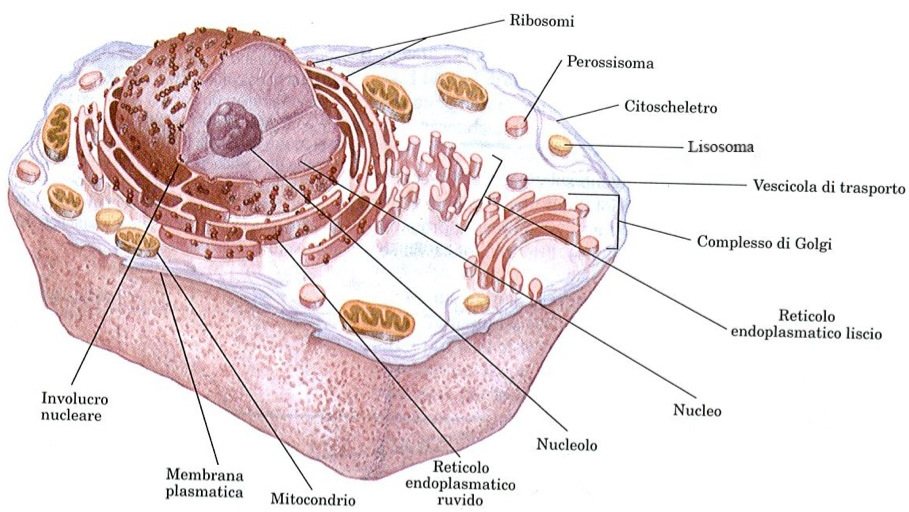
\includegraphics[width=10cm, keepaspectratio]{img/intro/cell.png}
\caption[The Cell]{Schematic representation of a cell.}
\label{fig:cell}
\end{figure}

\subsection{The DNA}
\label{sec:genica}
The \textit{DNA} was been isolated for the first time by the German doctor Friederick Miescher in 1869, while in the same decade the English biologist Charles Darwin was publishing \textit{On the Origin of the Species} and the  Augustinian friar scientist was communicating his results on the pees to the Brunn Natural History Society.

Because the substance isolated by Miescher was white, lightly acid and present only into the cells nuclei, it was been termed \textit{Nucleic Acid}.
Name modified afterwards in \gls{dna}, to distinguish is from the another one, very similar, the \gls{rna}.

These two molecules are constituted by \textit{nucleotides}, constituted by a nitrogen base, deoxyribose sugar and a phosphate group.
We distinguish two nitrogen bases, purines and pyrimidines.
Inside the \gls{dna}, we have two \textit{pyrimidines}, \textit{adenine (A)} and \textit{guanine (G)}, and two \textit{pyrimidines}, the \textit{Cytosine (C)} and the \textit{Thimine (T)}  .
Inside \gls{rna} \textit{Thymine} is substituted by the \textit{Uracil (U)}.

\begin{figure}[h]
\centering
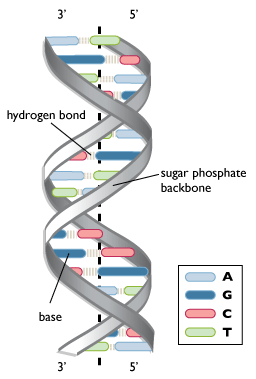
\includegraphics[width=5cm, keepaspectratio]{img/intro/dna1.png}
\caption[the \gls{dna}]{Schematic representation of double-stranded filament structure of \gls{dna}. The legend report the four nitrogen bases, Adenine, Guanine, Cytosine and Thymine.}
\label{fig:dna}
\end{figure}

\gls{dna} structure (figure \ref{fig:dna}) was discovered, in the 50's, by the American scientist James Watson, the French physicist Francis Crick and the English chemist-physicist Rosalind Franklyn.
According to their model the \gls{dna} is a double-stranded filament, where Adenines can pair only with Thymines and Guanines only with Cytosines.
The four bases constitute the alphabet for the genetic message.

\gls{dna} is folded on itself (\textit{\gls{dna} packaging}, thanks to specific "beads" called \textit{nucleosomes}, which themselves consist of eight proteins with tails, called \textit{histones}, that have the \gls{dna} wrapped on them.
This mechanism enables to store around 2 meters of chromatin inside a nucleus of a 2-10 micron diameter, when referring to Human specie.

Moreover, the \gls{dna} contains the \textit{genes}, particular sections containing relevant information for building proteins and other fundamental molecules for the cellular behavior regulation.
Each gene is localized on a precise position of a \textit{Chromosome}, which are in different number for each specie.
Each chromosome is constituted by \gls{dna} within thousands genes.

\begin{figure}[h]
\centering
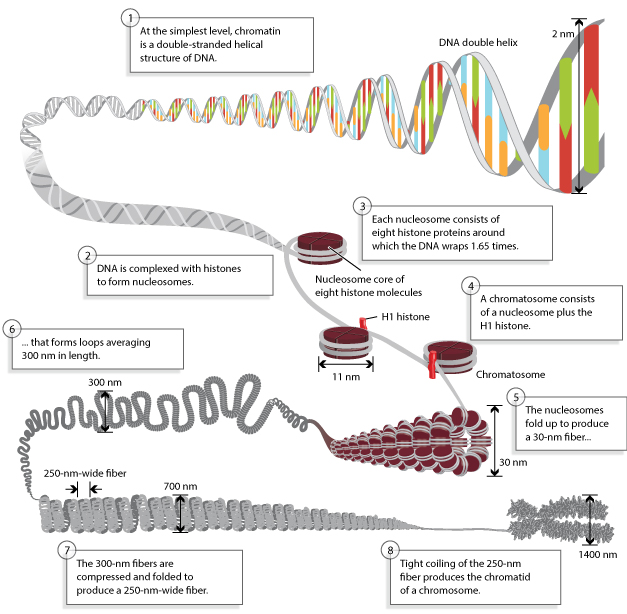
\includegraphics[width=8cm, keepaspectratio]{img/intro/dna2.jpg}
\caption[Chromosomes and \gls{dna}]{Representation of the relation between \gls{dna} and Chromosomes.
Inside the cell nucleus there are pairs of chromosome, constituted by chromatin, which fundamental unit is constituted by nucleosomes, on which the \gls{dna} is wrapped around, containing the genetic information in gene form. (image adapted from \cite{Annunziato2008})}
\label{fig:dnachromosome}
\end{figure}

Figure \ref{fig:dnachromosome} better helps  to understand the relationship between chromosomes, chromatin, nucleosomes and genes.

It is important to underlying that since some decades ago the Central Dogma of Molecular Biology was founded on the transcription - translation principle, where \gls{dna} was transcribed in \gls{rna}, which subsequently it would have been translated into protein.

Nowadays, we know that the gene transcription is regulated by several mechanisms, and moreover, the translation is not the only process fated for \gls{rna}.

Indeed, for a transcription of a gene, there are some requisites to be respected, such as the accessible of that specific part of the chromatin, or the binding of specific proteins enabling the accession to the gene region, or the histone modification processes, such as \textit{Acetylation}, \textit{Methylation}, \textit{Phosphorylation}, and others, which modifies the state of specific histones, and influencing gene expression regulation. 
  
\begin{figure}[h]
\centering
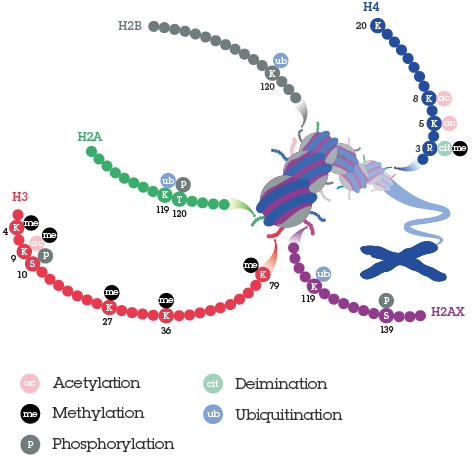
\includegraphics[width=8cm, keepaspectratio]{img/intro/hm.png}
\caption[Histon modification]{Representation of some processes involved in histone modification, influencing gene expression regulation.}
\label{fig:histmod}
\end{figure}


\section{Sequencing Techniques}
\subsection{RNA-Seq} \label{sec:rnaseq}
textit{RNA-Seq} \cite{Thermes2014, Wang2009, Costa2010, Ozsolak2011} is the most widely used technology to understand gene related regulatory mechanisms in response to stress conditions or drug treatments and progressions of several diseases \cite{Costa2013}.

The main aim of RNA-Seq experiment is to highlight the mainly altered processes (either up-regulated or down-regulated) when comparing two or more conditions at a specific instant in time or in subsequent time points (time-course experiment), and then identify the biological mechanisms regulating such changes.

The general idea underlying the library preparation of an RNA-Seq experiment can be viewed as the conversion of long mRNAs segments in cDNA fragments with RNA or DNA fragmentation. 
To each sequence an adapter for the sequencer is added and a short read is obtained with high-throughput sequencing technology (Figure \ref{fig:rnaseqexp}).


\begin{figure}[h]
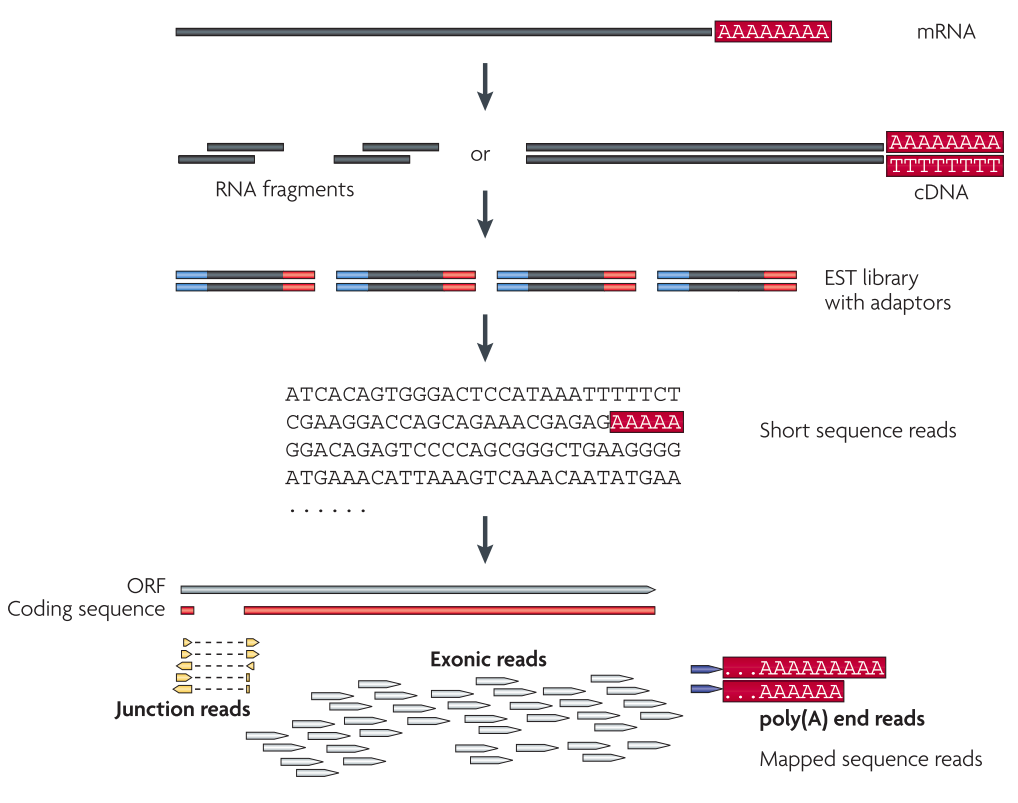
\includegraphics[width=\textwidth,height=\textheight,keepaspectratio]{img/intro/rna-seq.png}
\caption[RNA-Seq experiment]{Representation of an RNA-Seq experiment. \cite{Wang2009}}
\label{fig:rnaseqexp}
\centering
\end{figure}

In order to investigate the experiment, the so-obtained reads have to be analyzed with several tools depending on the particular question the researcher is interested in \cite{Pepke2009, Oshlack2010}.

\begin{figure}[h]
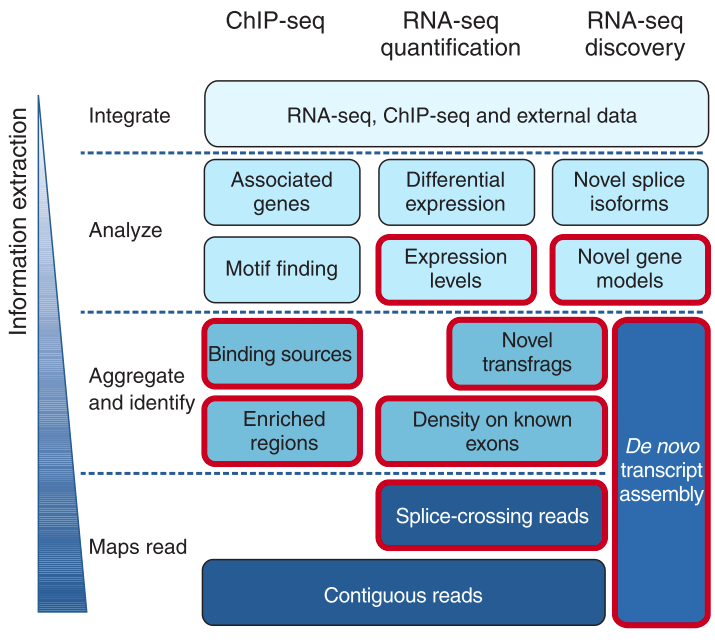
\includegraphics[width=\textwidth,height=\textheight,keepaspectratio]{img/intro/rna-seqan.png}
\caption[RNA-Seq analysis]{Representation of the possible complexity of RNA-Seq analysis. \cite{Pepke2009}}
\label{fig:rnaseqan}
\centering
\end{figure}

In particular we focused on the RNA-seq quantification in case of multiple biological conditions, due to stress, drug treatments, disease specific, etc. where a typical analysis starts from the alignment of the reads on a specie reference genome and the quantification of the mapped reads, producing a count matrix of the samples (on columns) and the genes related features (on the rows), typically identifiers depending on the annotation database used by the analyzer.
Commonly, the counts matrix needs to be filtered from low expressed features and then normalized across the samples, to reduce specific bias for each sample.
Then, it is possible to choose between several methods for the detection of differential expression of the features between the conditions (see section \ref{sec:ticorsermethods}).
Finally, the significant features can be integrated with databases of biological functionalities in order to detect the mostly influenced ones.


\subsection{Atac-Seq} \label{sec:atacseq}
The chromatin packaging of the genome plays a fundamental role in gene regulation of eukaryotic individuals.
To study this aspect of the \gls{dna} several technologies have been developed, such as \textit{FAIRE-seq} \cite{Giresi2007}, \textit{DNase-seq} \cite{Winter2013} and \textit{ATAC-seq} \cite{Buenrostro2013}, etc.

\textit{ATAC-seq} among the others is having a growing interest and diffusion in the last years, because it offers comparable results to the DNASE-seq with less biological material and less library preparation time.

\begin{figure}[h]
\centering
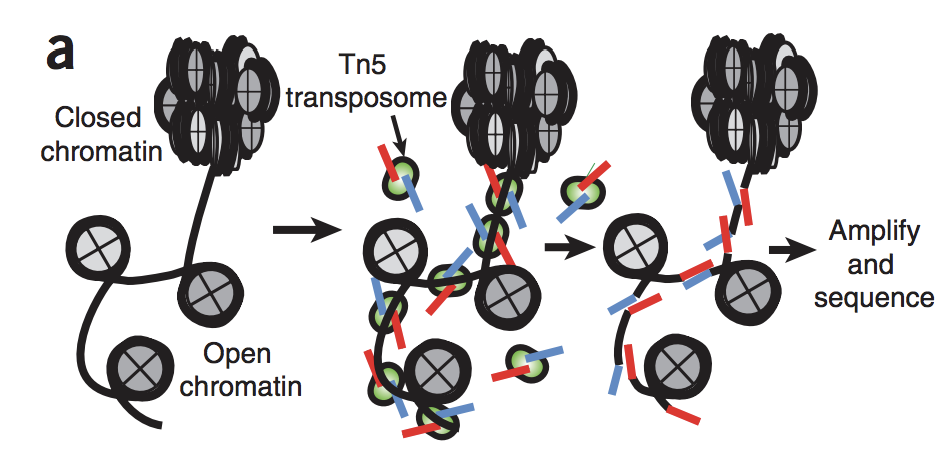
\includegraphics[width=9cm,keepaspectratio]{img/intro/atac.png}
\caption[ATAC-seq experiment]{Representation of ATAC-seq library preparation. \cite{Buenrostro2013}}
\label{fig:atacseqexp}
\end{figure}

The library preparation adopts a hyperactive Tn5 transposase, modified with adaptors for high-throughput  \gls{dna} sequencing, which is able to fragment and tag a genome simultaneously.
The technology exploit the Tn5 capability of integrating itself into active regulatory elements.

After Tn5 tagmentation, the resulting segments can be amplified and sequenced, producing sequences to map on a reference genome.
There is no standard analysis reached for the ATAC-seq analysis, but, inspired by the \textit{ChIP-seq} analysis, the resulting reads, typically, are processed with tools (peak callers) for quantifying their amplification, which produces for each detected open chromatin region a feature, the peak (generally with an associated score). 

Depending on the used tool, the peaks can be represented in different data structures, but their representation is given by the genomic coordinates; chromosome, starting and ending point of the region, the strand of the DNA on which the region lies, and additional attributes such as a score, a number of samples on which the regions has been detected, etc.

To obtain a first level of integration, the peaks can be annotated with other relevant features of the genome, such as the \gls{tss} of the genes, \gls{utr}, promoters, exons, introns, etc.  
Then, the annotated genes can be used to enrich for GO terms or pathways, reaching a second level of integration.






\section{Computational Aspects}


\chapter{TiCoRSe - Time Course RNA-Seq data analysis}
\section{Introduction}
\subsection{Time Course RNA-Seq}
\section{Methods}
\subsection{General Approach}
\subsection{Time Course Methods}
\subsection{Other Methods}
\subsection{Additional Features}
\section{Results}


\chapter{DEScan2 - Differential Enriched Scan 2} \label{sec:descan2cap}

\textbf{\textsl{few words on integration of epigenomic with transcriptomic}}

To investigate and answer epigenetic biological questions we decided to create a useful instrument for analysing epigenomic data (such as \textit{ChIP-Seq}, \textit{Atac-Seq}, \textit{Sono-Seq}).
Very often the biological questions to be answered, as for the RNA-Seq, need the comparison of two or more different biological conditions.
Starting from a set of already published \cite{Koberstein2018} scripts, we designed \textit{Differential Enriched Scan 2} (\textit{DEScan2}), a software for helping the analysis of epigenomic data.

\section{Introduction} \label{sec:descan2intro}
In order to deeply understand and reconstruct cellular mechanisms influenced by drug treatments, pathologies or diseases, it is fundamental to look at multiple omics data types at the same time.

Previous chapters deeply described tools for multiple omics data analysis, integration and visualization using command line tools.
Even if the command line approach is pretty common inside the bioinformatics community, it is not for every scientist who is not so confident with programming languages or terminal.
When working with multiple omics data, there is an overabundance of available tools for each sequencing that can bewilder a beginner, up to the point to renounce approaching the analysis problem.

%Moreover, thanks to our previous experiences \cite{russo2015advantages} in developing \gls{gui}, we noticed a growing interest by the scientific community in using interactive software.
%This interest seems to be leaded by multiple motivations, such as the need to analyze data very fast or the lack of time in learning programming languages and terminal-line based tools.

Furthermore, even if the bioinformatics community has massively moved on the development of novel statistical and computational methods for multi-omics data integration, part of the scientific community is still anchored to the single-omics analysis side.
Even if still really helpful, it is still very common to read published papers based on single-omics data analysis without taking into account possible integrated solution with other omics data types.

Of course, it is not so simple to afford for multiple omics data experiments, but, nowadays, the internet swarms of public datasets.
In particular when looking at public biological data banks, such as \gls{geo}\footnote{\url{https://www.ncbi.nlm.nih.gov/geo/}} \cite{Services2007} or \gls{tcga}\footnote{\url{https://cancergenome.nih.gov/}} \cite{tcga2013a}, where it is possible to retrieve as many data as needed.

On the other side, if there are not so many papers publishing integrated analysis, it is also difficult for analysts to retrieve the right methodologies for the multi-omics data analysis and their visualization. 

\begin{figure}[H]
\centering
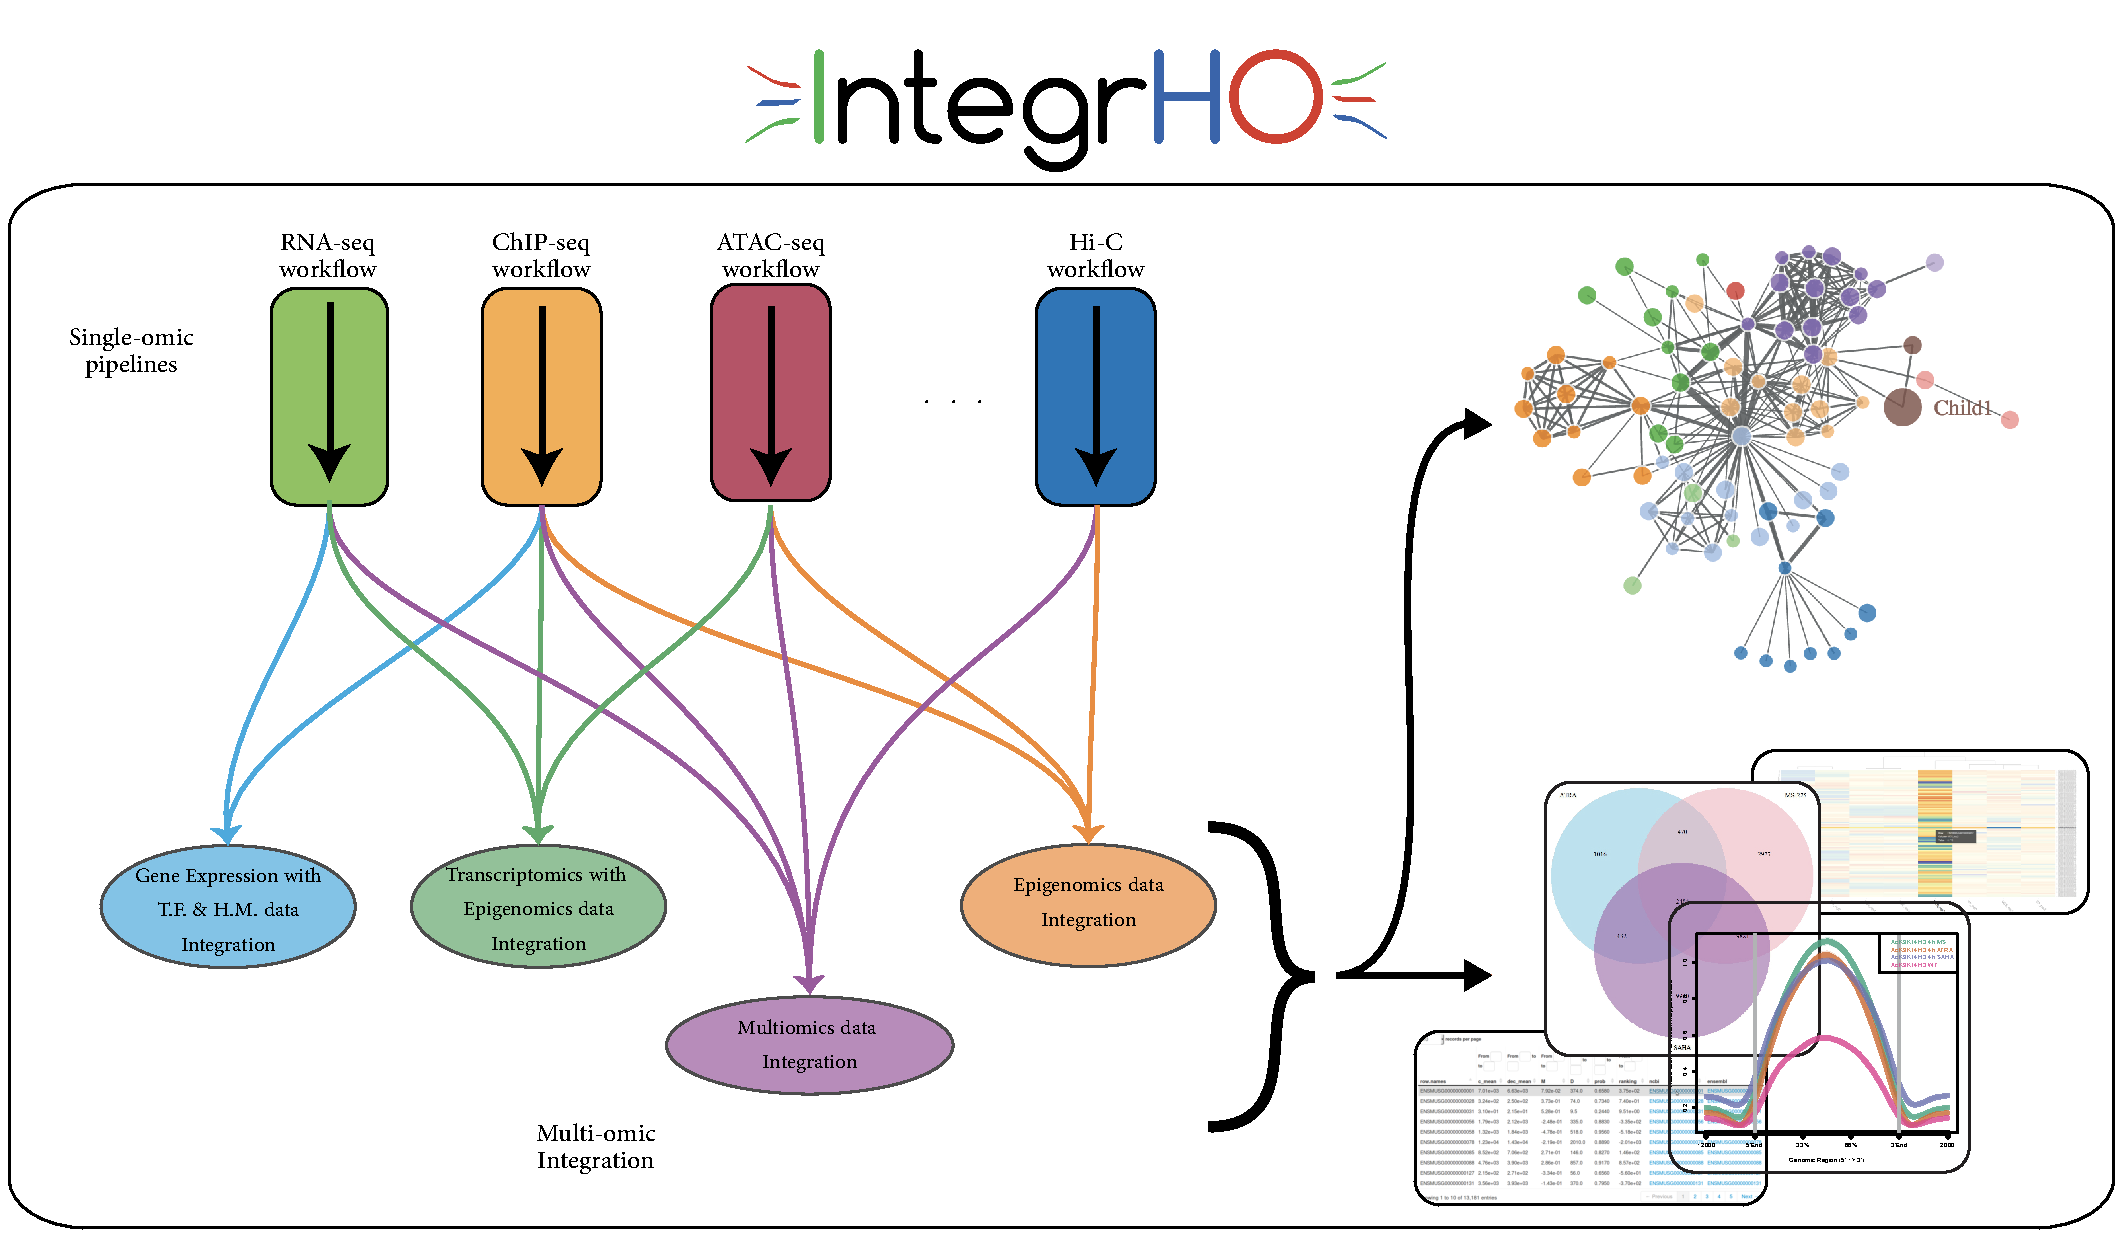
\includegraphics[width=\textwidth, keepaspectratio]{img/integrho/integrho_scheme.pdf}
\caption[\gls{igro} representation]{A schematical representation of \gls{igro} underlying idea.
Single-omics analysis methods are proposed in order to facilitate their multiple integration.
This integration can lead to produce graphical results, in case of low dimension datasets, or to more sophisticated integration model such as regulation networks, in case of high-dimension datasets.}
\label{fig:integrhoidea}
\end{figure}

Based on these considerations and in order to promote the multi-omics data integration, we decided to provide the scientific community of a novel easy-to-use instrument which not only gives the possibility to analyze single-omics data types but also guides the user through multiple ways of integrating multi-omics data types (figure \ref{fig:integrhoidea} gives an underlying idea of \gls{igro}).





%Several interface-based tools \cite{Poplawski2016} have been proposed during last years but too often they are oriented to analyze singular-omics or when designed for multi-omics, they are pipeline oriented. 

%In this chapter we introduce \gls{igro}, our web-based platform for multi-omics data analysis and integration,  in a \gls{rr} spirit.




\section{Methods} \label{sec:descan2methods}
Here we present \textit{easyReporting}, an \textit{R6} \footnote{\url{https://adv-r.hadley.nz/r6.html}}\footnote{\url{https://cran.r-project.org/web/packages/R6/index.html}} class\footnote{\url{https://en.wikipedia.org/wiki/Class_(computer_programming)}} developers to integrate a reproducible research layer inside their software products, as well as lazy analysts to speed up their report production without learning the \textit{rmarkdown} language.

In such a way, thanks to minimal additional efforts of developers, the end user has available an \textit{rmarkdown} file within all the source code generated during the analysis, divided into \glspl{cc} ready for the compilation.

Once manually edited with comments and descriptions the file can be compiled to produce an enriched document within input data, source code and output results.

A so final document can be attached to the publication of the analysis as supplementary material, helping the interested community to entirely reproduce the computational part of work (figure \ref{fig:rrscheme}). 

The package is accessible at the following link:\\ \href{https://github.com/drighelli/easyreporting}{https://github.com/drighelli/easyreporting} 

\subsubsection{General Description and Initialization}

The class can to be imagined as a schematic representation of the \textit{rmarkdown} file (\textit{report}), indeed 
its attributes represent the \textit{report} characteristics, which are typically inserted in the header of the file.
But our class methods are not only for the attributes manipulations but also for insertion of \glspl{cc}, comments and section titles inside the \textit{report}.

As any typical class, before of using it, \textit{easyReporting} requires to be initialized with the \lstinline!new! command, passing as mandatory arguments the \textit{path} and the name of the file as \lstinline!filenamepath! and a title as \lstinline!mainTitle!.
Additionally, an \lstinline!author! and the \lstinline!documentType! can be specified.

When initializing, the class automatically creates the \textit{report} with the entire specified folder tree, setting up the header of it and declaring the general options for the \textit{rmarkdown} file.
If \textit{rmarkdown} personal options (see figure \ref{fig:knitropts} for a list of available options) are required, before creating an instance of the class, it is possible to use the \lstinline!makeOptionsList! function, and then assigning the output to the \lstinline!optionsList! argument of the class \lstinline!constructor!.

\begin{figure}[H]
\centering
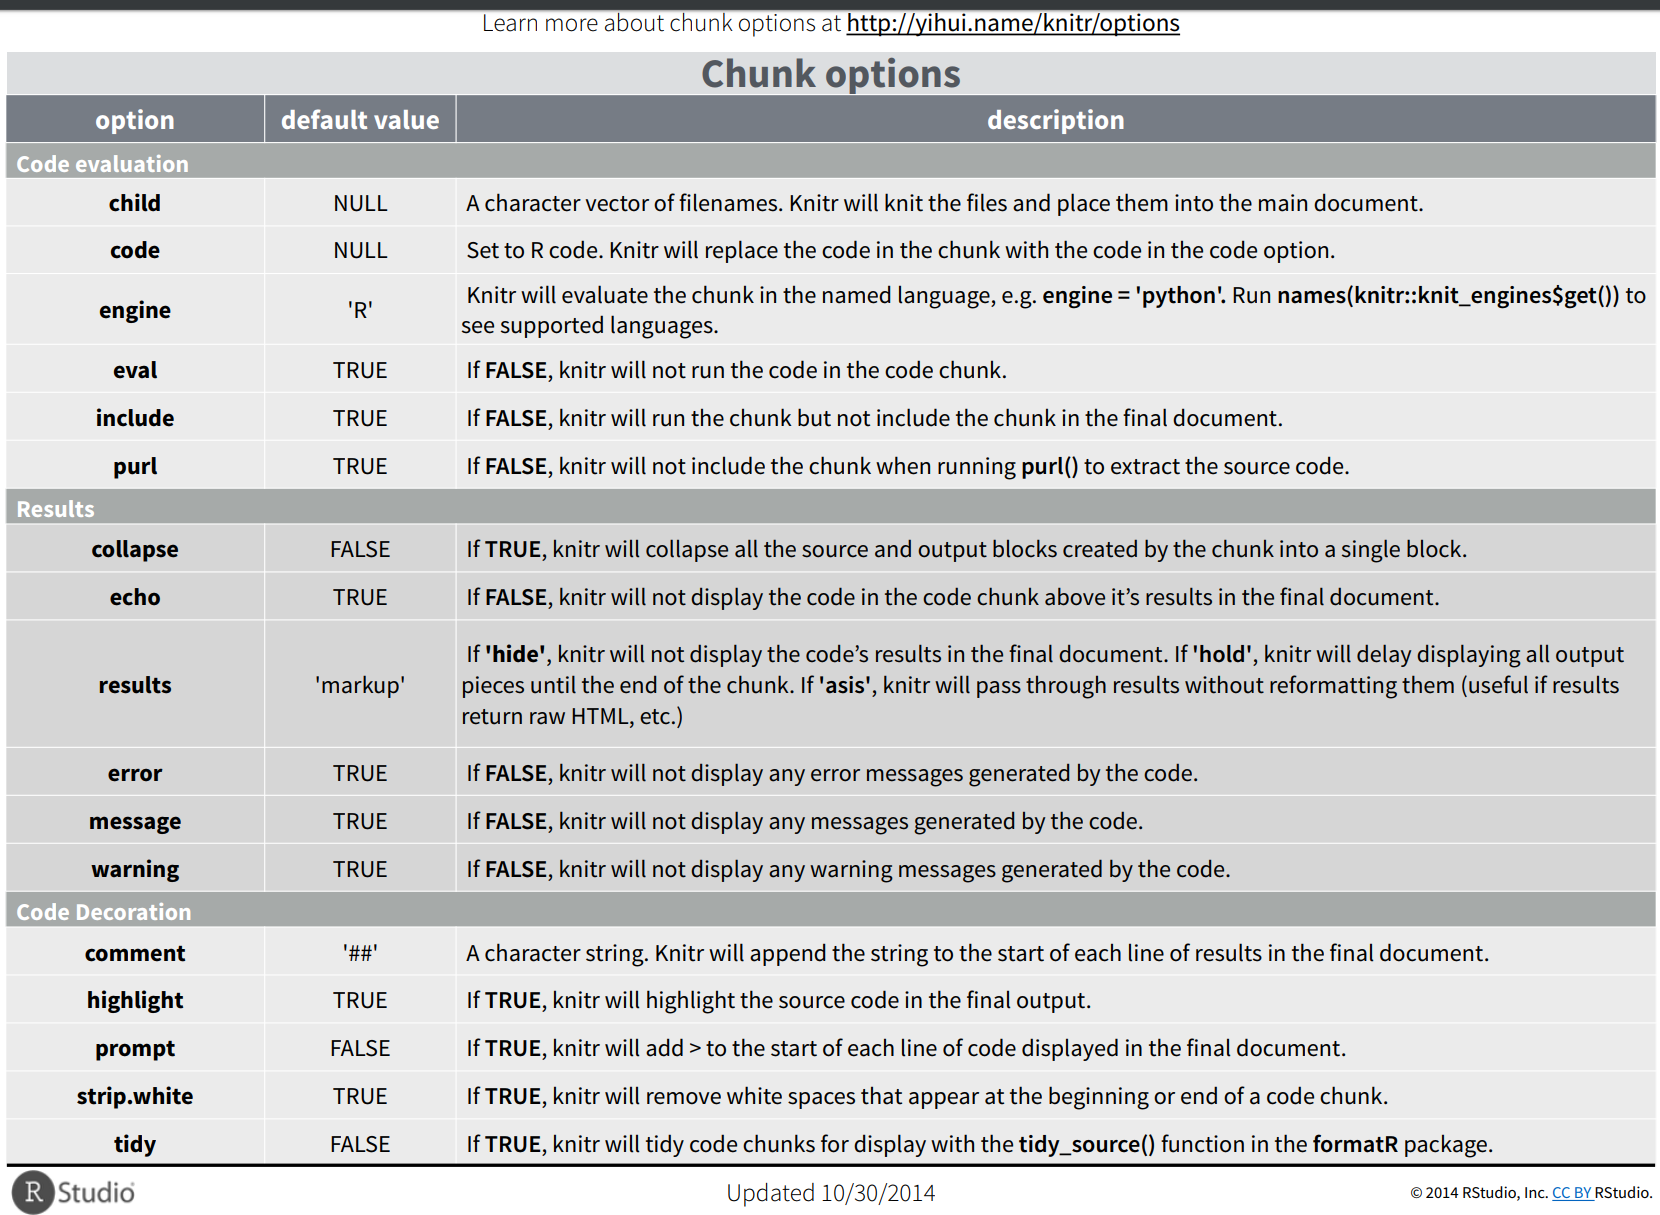
\includegraphics[width=\textwidth, keepaspectratio]{img/rr/knitropts.png}
\caption[knitr options]{A schematic table of options available using knitr and rmarkdown packages.}
\label{fig:knitropts}
\end{figure}


\subsubsection{Class Methods}

The class is provided of several methods for \textit{rmarkdown} \gls{cc} construction.

Once an \textit{easyReporting} instance is available, with \lstinline!mkdTitle! it is possible to insert six levels of titles, by setting the parameters \lstinline!title! and \lstinline!level!.
It is also possible to add natural language comments with \lstinline!mkdGeneralMsg!.

When working with \glspl{cc}, two main choices are available.
The first one gives the possibility to construct a \gls{cc} as additional steps, by using first the \lstinline!mkdCodeChunkSt!, then adding variable assignment and/or function calling with \lstinline!mkdVariableAssignment! or \lstinline!mkdGeneralMsg!, and finally closing the \gls{cc} with \lstinline!mkdCodeChunkEnd!.

In particular, when starting a \gls{cc} with \lstinline!mkdCodeChunkSt!, it is possible to assign a specific \lstinline!optionList! and/or a \lstinline!source.files.list! to be added to that \gls{cc}.

Otherwise it is possible to create an entire \gls{cc} just with \lstinline!mkdCodeChunkComplete! and assigning the entire function call as a \lstinline!message!.
This way of working is really useful with \lstinline!function! creation, where inside a developed function a simple recursive call with parameters assignment can be done as a single \lstinline!message!.






\subsection{Peak Caller} \label{sec:descan2peakcall}
However, the package can work with any external peak caller returning results in terms of bed files, indeed the package provides additional functionalities to load bed files of peaks and handle them as GenomicRanges \cite{Lawrence2013} structures.


\subsection{Peak Filtering and Alignment} \label{sec:descan2filtering}

In order to filter out false positives peaks, we designed a method (\lstinline{finalRegions}) which firstly filters out low score regions and then aligns the resulting regions between the samples, using two different thresholds.
One on the peaks's score and one on the number of samples.

The filtering step is designed to take as input a list of peaks as \textit{GenomicRangesList}, where each element represents a file.
This is the data structure produced by the peak caller, but, we also developed a method to load peaks produced by other software like MACS \cite{Zhang2008}, as described in section \ref{sec:descan2addfeat}.

Firstly, using the threshold on the peaks's score (\lstinline{zThreshold} parameter), the method filters out the peaks with a score lower than the user-defined threshold value.

Then, for aligning the peaks between the samples, it extends a 200bp window in both directions of remaining regions, computing the overlaps using the \lstinline{findOverlapsOfPeaks} method (with \lstinline{connectedPeaks} parameter set as \lstinline{merge}), as defined in \textit{ChIPpeakAnno} \cite{Zhu2010} R/Bioconductor package.

Based on this idea, the filtering step is developed to filter out those peaks not present in at least a user-defined (\lstinline{minCarriers} parameter) number of samples. In the light of this, the user can decide the minimum number of samples where each peak has to be detected.
On our experience, we suggest to set the samples threshold as a mutiple of the number of replicates of the conditions.



\subsection{Peak Counts} \label{sec:descan2peakcounts}
The counting step (\lstinline{countFinalRegions} method) is designed to take a \textit{GenomicRanges} data structure as input, where for each peak additional features, as the score and the number of samples, are saved.
Moreover, it requires also the path of the BAM/BED files where the reads are stored, in order to quantify the peaks given as input.

For each region the method counts the number of reads present in each sample.
In so doing, it produces as result a matrix of the counts, where the rows and the columns represent, respectively, the regions and the samples.

In order to keep trace of all information associated to the regions, it produces a \textit{SummarizedExperiment} \cite{SummExp} data structure, giving the possibility to retrieve the \textit{GenomicRanges} peaks associated data structure and the count matrix, respectively, with \lstinline{rowRanges} and \lstinline{assays} method.

The choice to produce a count matrix is guided by the versatility of this data structure, useful not only for the differential enrichment of the regions between multiple conditions, but also for integrating the epigenomic data with other -omics.

\subsection{Additional Features} \label{sec:descan2addfeat}
The package offers additional features for loading data (i.e. peaks) resulting from other sources, and for manipulating \textit{GenomicRanges} data structure.

The method \lstinline{readFilesAsGRangesList} takes as input a directory with BAM or BED data, to load in \textit{GenomicRangesList} format.
This data structure is useful to store genomic information, as peaks or mapped reads, produced by other software like \textit{MACS2} or \textit{STAR} and, in case of peaks, it is necessary during the \gls{descan} filtering step.
Additionally to \lstinline{fileType} (BAM, BED, BED.zip) parameter specification it requires the genome code to use during the file processing.
Moreover, when the input files represent peaks the \lstinline{arePeaks} flag needs to be set to \lstinline{TRUE}.
In such a way the \gls{descan} package can work also with data coming from other sources, preferred by the user.

Furthermore, \gls{descan} provides several functionalities for GenomicRanges data structure
handling. One over the others (\lstinline{fromSamplesToChrsGRangesList}) gives the possibility to split a GenomicRangesList by the chromosomes. 
This procedure could be useful for parallelizing the computations on the chromosomes, assigning a single chromosome to a single computing unit.
Taken as input a GenomicRangesList organized by samples, this method returns a list of chromosomes, where each element has a GenomicRangesList of samples, containing only the regions associated to the single chromosome.

[Create figure to better explain the transformation]

Other useful utilities are \lstinline{keepRelevantChrs}, that takes a GenomicRangesList and a list of chromosomes and return only the interested chromosomes.
\lstinline{saveGRangesAsTsv} that saves a tab separated value file starting from a GenomicRanges.
\lstinline{saveGRangesAsBed} that save a standard BED file format starting from a GenomicRanges data structure.
\lstinline{setGRangesGenomeInfo} which, starting from a genome code, sets a specific \textit{genomeInfo} to a \textit{GenomicRanges} object.

\section{Case Study} \label{sec:descan2results}
\textbf{Few words on ATAC-Seq data}

We illustrate the performances of \gls{descan} using a dataset \cite{Su2017} that describes in vivo adult mouse dentate granule neurons before and after synchronous neuronal activation using Atac-Seq and RNA-Seq technologies (see sections \ref{sec:atacseq} and \ref{sec:rnaseq} for a description of these sequencing techniques).

This dataset is organized in 62 samples of Atac-Seq and RNA-Seq, extracted at different time points, with four replicates at each time point.
We chose to compare the differences btween the first two stages, time 0 (E0) and 1 hour after neuronal induction (E1), in order to show a possible Atac-Sec workflow for Differential Enrichment, and how to integrate this data type with RNA-Seq. A general illustration of our dataset is represented in figure \ref{fig:atacdataset}.

\begin{figure}[H]
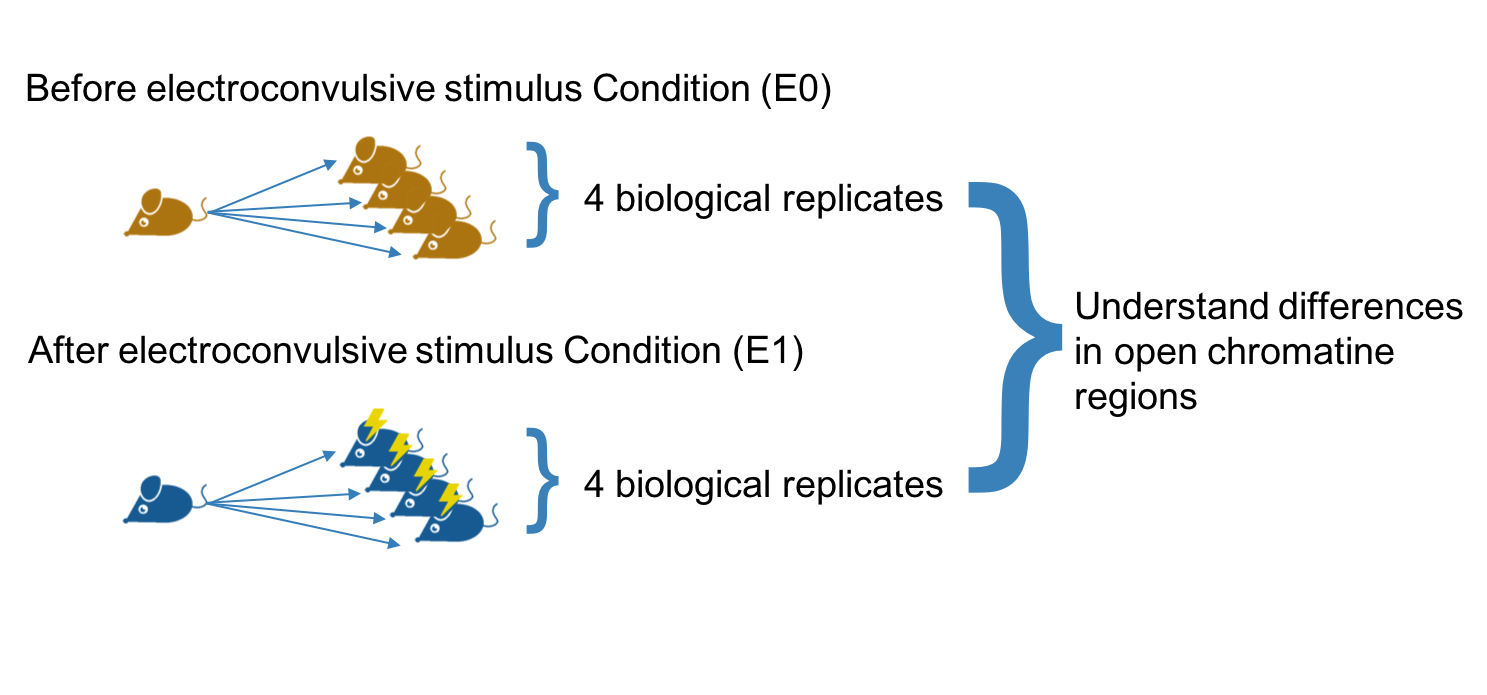
\includegraphics[width=\textwidth,height=\textheight,keepaspectratio]{img/descan2/dataset.png}
\caption[DEScan2 dataset illustration]{An illustration of our extraction of the \cite{Su2017} dataset.}
\label{fig:atacdataset}
\centering
\end{figure}

We downloaded the data from \gls{geo} database \cite{Edgar2002, Barrett2013} with accession number GSE82015\footnote{\url{https://www.ncbi.nlm.nih.gov/geo/query/acc.cgi?acc=GSE82015}} and mapped raw data using \textit{STAR} \cite{Dobin2013} with default parameter on \gls{mm10}.

In order to detect the open chromatin regions we run our peak caller, cutting the genome in bins of 50bp and using running windows of minimum 50bp and maximum 1000bp. In such a way we are able to detect not just broad peak, but also smaller peaks.

To be confident with our results we compared the \gls{descan} detected peaks with the same validated regions (Arc and Gabrr1) in the original work \cite{Su2017}.
The lower part of figure \ref{fig:peaksdescan} shows the detected and validated regions (in blue and red) resulting differentially enriched between the E0 (in pink) and E1 (in green) conditions, while the upper part shows \gls{descan} peaks (in blue), highlighting a capability to catch not only the same regions of the published ones, but also (gold circles) to be more careful in the smaller peaks detection.

\begin{figure}[H]
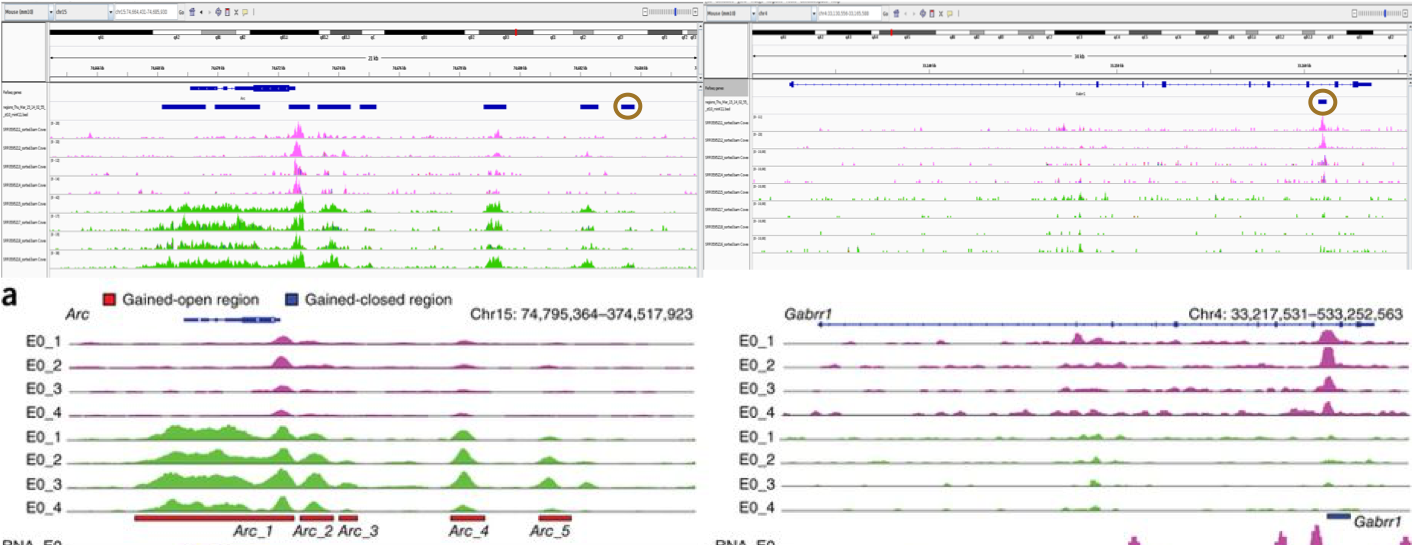
\includegraphics[width=\textwidth,height=\textheight,keepaspectratio]{img/descan2/peaks.png}
\caption[\gls{descan} peaks detection]{A comparison of \gls{descan} detected peaks with validated peaks in article \cite{Su2017}.}
\label{fig:peaksdescan}
\centering
\end{figure}

Moreover, we run \textit{MACS2} on the same samples, and (as shown in figure \ref{fig:des2m2peaks}) \gls{descan} seems able to catch much more peaks than \textit{MACS2} for each sample.

\begin{figure}[H]
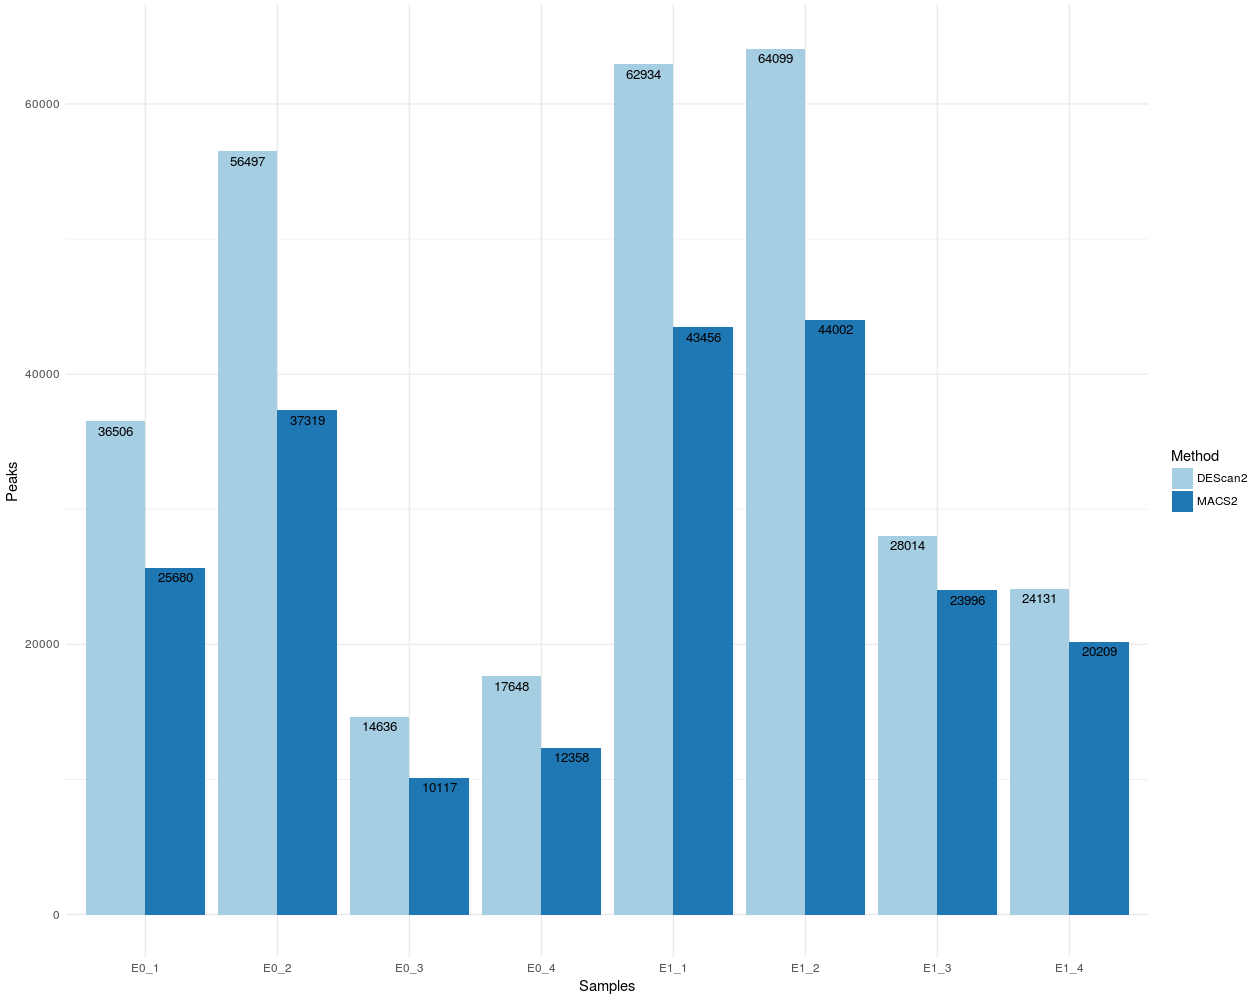
\includegraphics[width=\textwidth,height=\textheight,keepaspectratio]{img/descan2/d2m2_peaks_number.png}
\caption[The \gls{descan} and \textit{MACS2} peaks detection]{A comparison of \gls{descan} and \textit{MACS2} detected peaks for each sample in the dataset.}
\label{fig:des2m2peaks}
\centering
\end{figure}

While it is very important to detect good peaks with a peak caller, it seems to be more relevant to detect reliable regions. Indeed, during the filtering step, the number of peaks depends not only by the peak score, but also by the number of replicates designed in the experiment.
The figure \ref{fig:filteringdescan} puts in relation these two relevant information. 
On the x-axis is represented the number of replicates, while on the y-axis is traced the number of peaks, and each curve represents a different threshold on the peaks score, showing that higher are the thresholds on the scores and the number of replicates, lower is the number of the detected peaks.
Highlighting a proportional inversion between the number of the peaks and the combination of the number of samples and the detected regions score.


\begin{figure}[H]
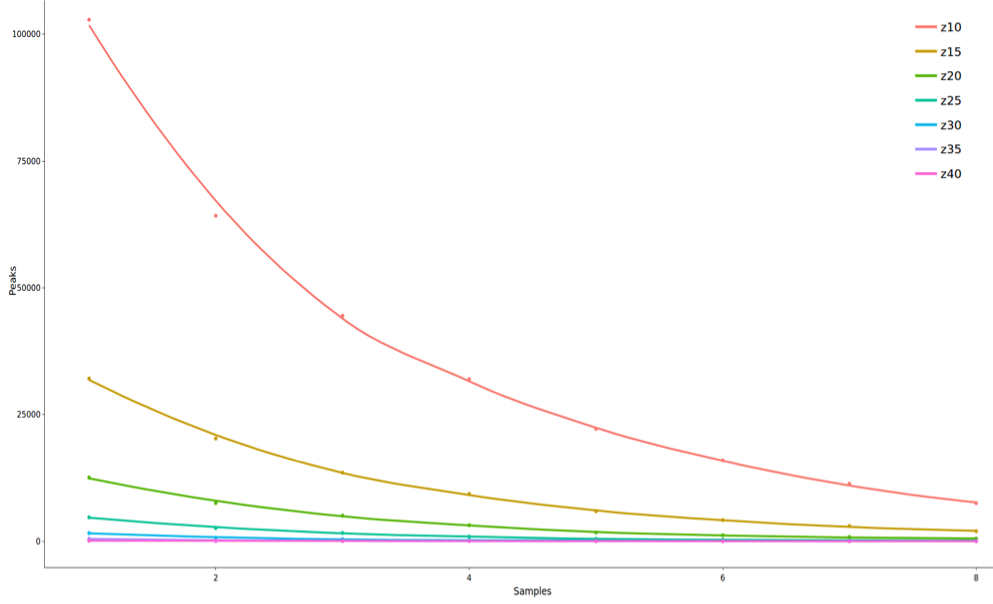
\includegraphics[width=\textwidth, height=\textheight, keepaspectratio]{img/descan2/filtering.png}
\caption[\gls{descan} filtering step]{Filtering the detected regions with different thresholds on peak scores.}
\label{fig:filteringdescan}
\centering
\end{figure}


\begin{figure}[H]
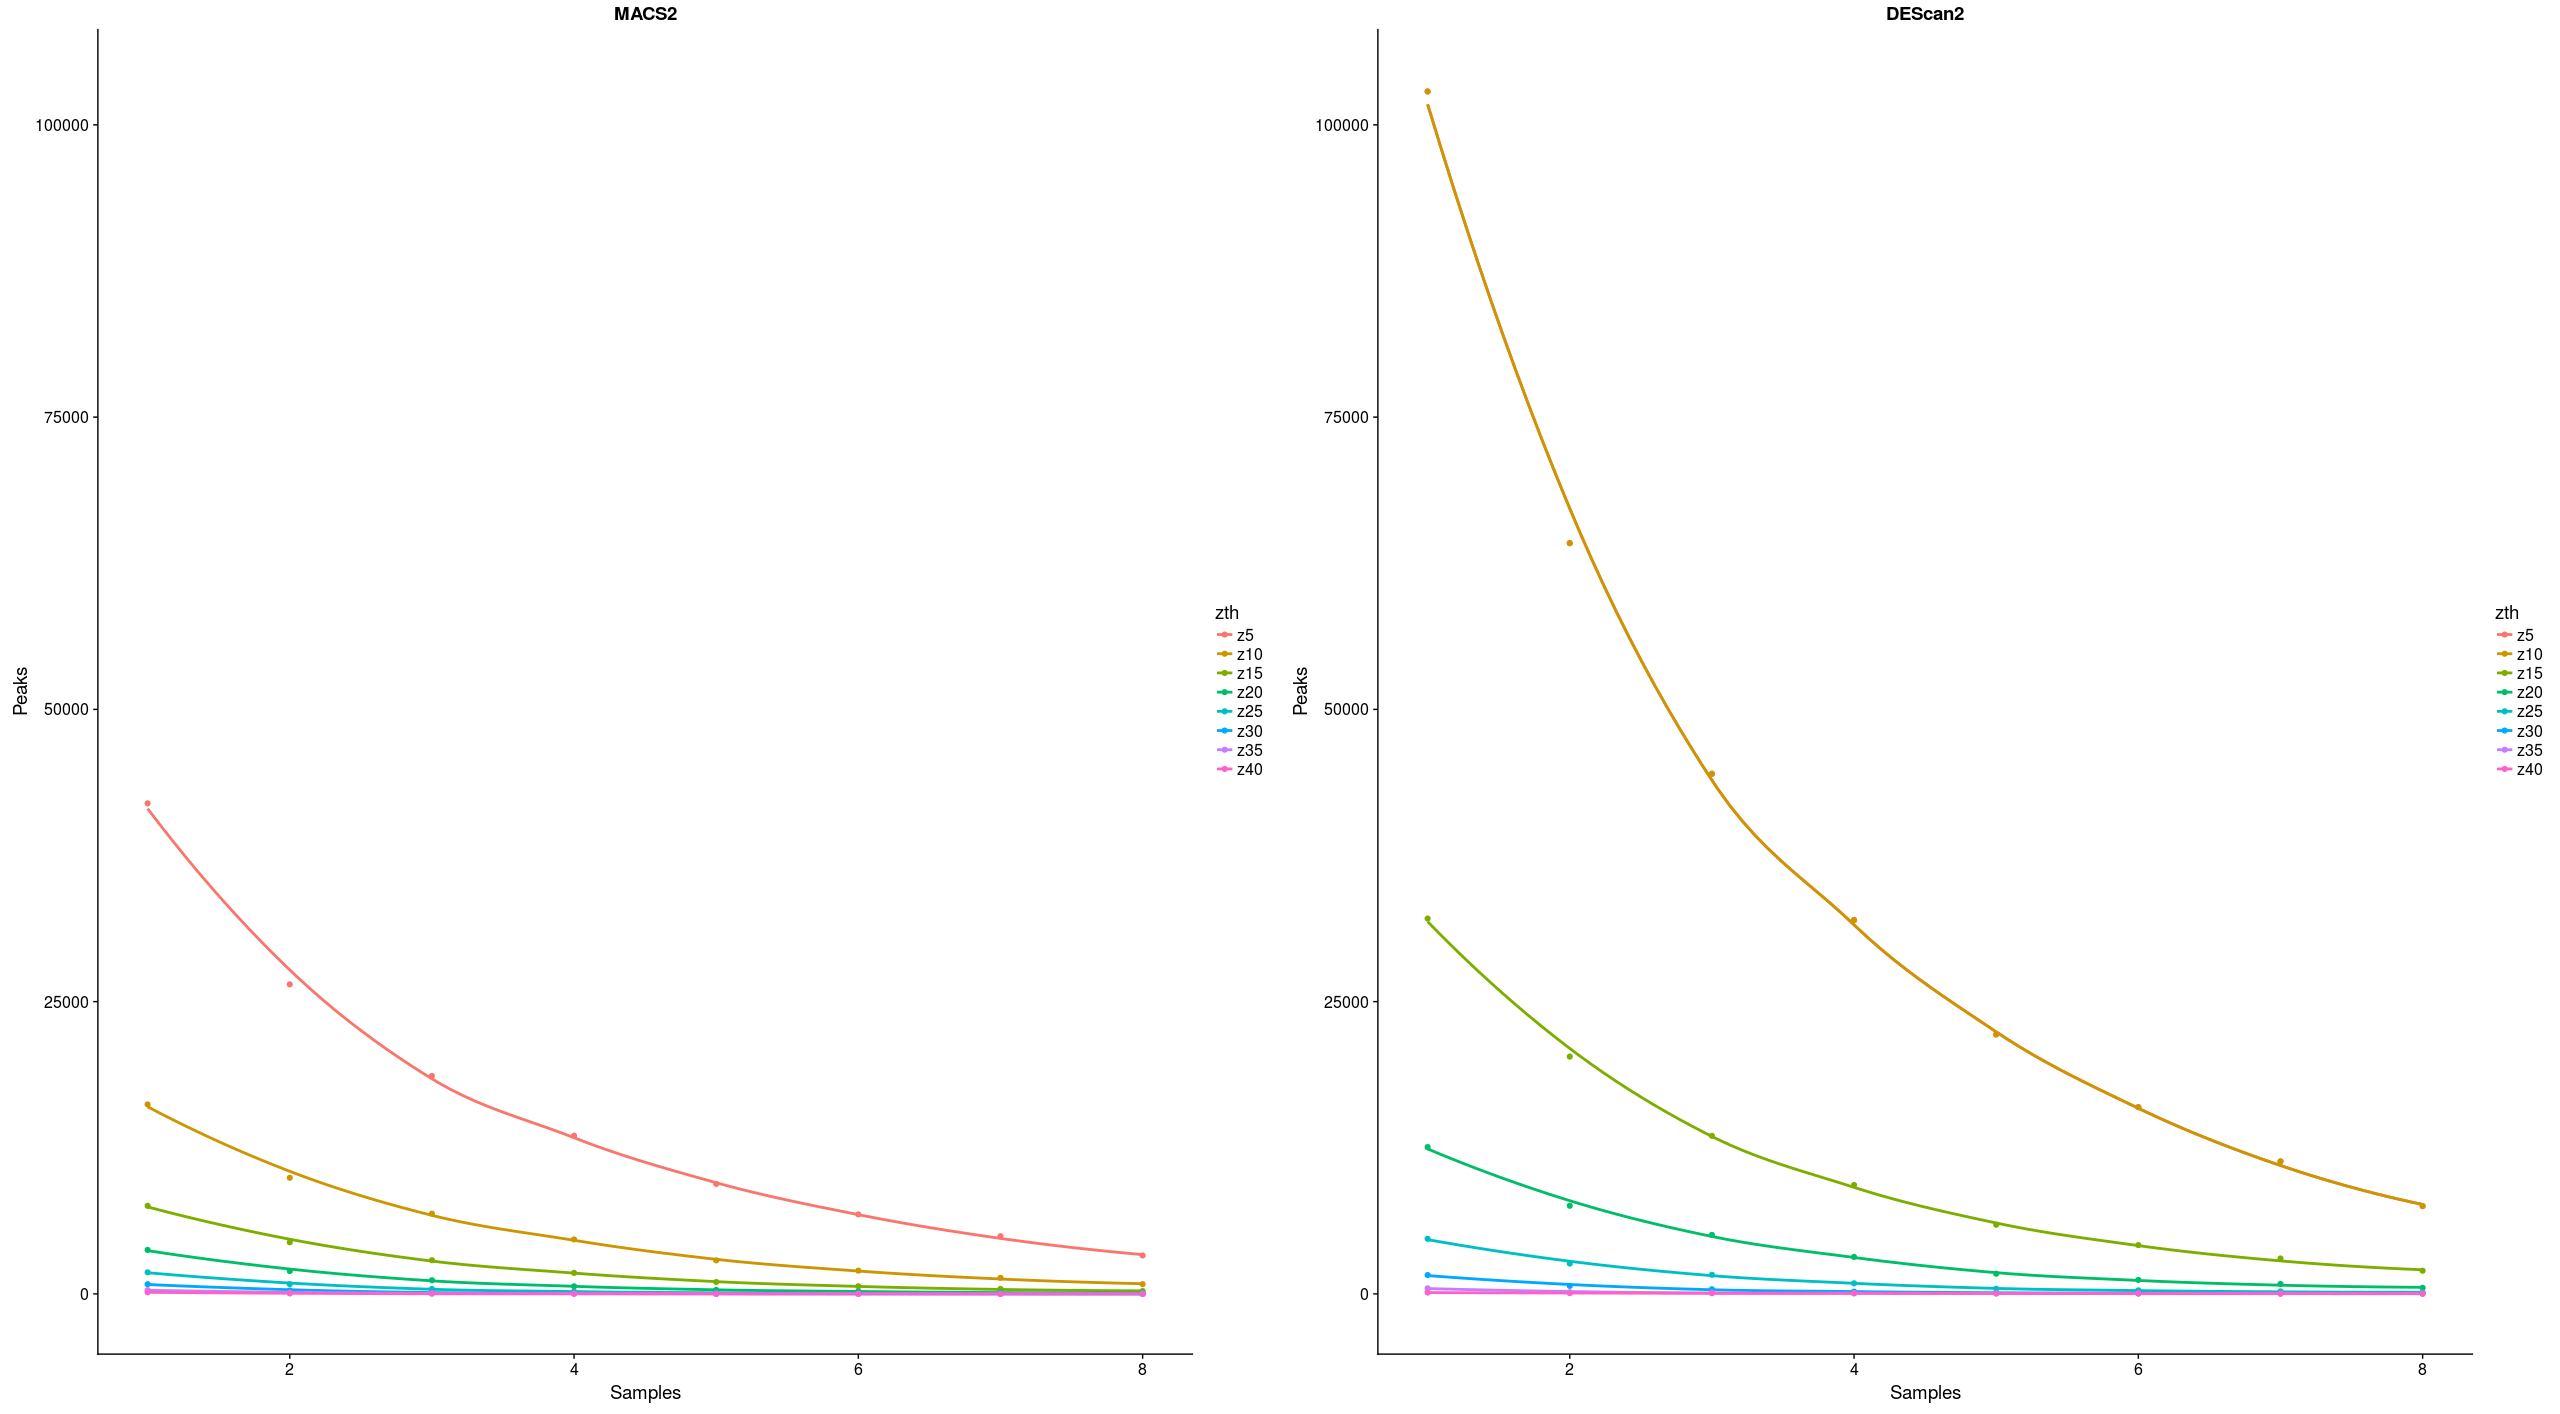
\includegraphics[width=\textwidth, height=\textheight, keepaspectratio]{img/descan2/filtering_m2_d2.png}
\caption[\gls{descan} and \textit{MACS2} filtering comparison]{Filtering the detected regions with different thresholds on peak scores between \textit{MACS2} and \gls{descan}.}
\label{fig:filteringdescanmacs2}
\centering
\end{figure}

The filtered-in regions can be processed by \gls{descan} in order to obtain a count matrix with samples on the columns and peaks on the rows.
This type of data structure is very versatile, because it enables to perform several operations, like the \glspl{der} and, if possible, the integration with other kind of omics, as RNA-Seq.

In order to preserve the information associated to the peaks, \gls{descan} produces as output a \textit{SummarizedExperiment} (figure \ref{fig:countsdescan}) data structure, which enables to retrieve the count matrix with \lstinline{assays} method, and to access the peaks information in \textit{GenomicRanges} format with the \lstinline{rowRanges} method. %{

\begin{figure}[H]
\centering
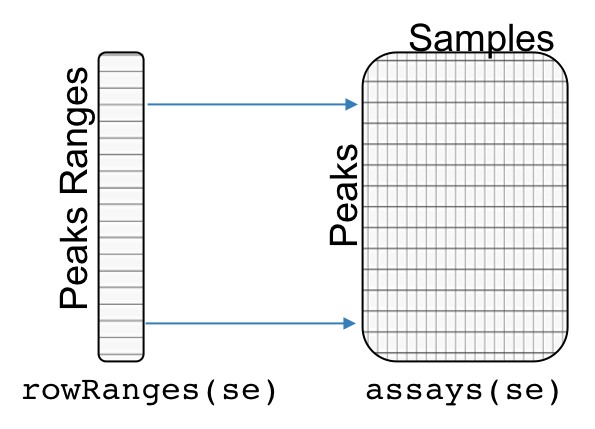
\includegraphics[keepaspectratio]{img/descan2/counts.png}
\caption[\gls{descan} counts illustration]{An illustration of the \textit{SummarizedExperiment} data structure produced by \gls{descan}.}
\label{fig:countsdescan}
\centering
\end{figure}

Before to proceed to detect \glspl{der}, it is a good standard to normalize the data, also because without any kind of normalization we are not able to detect any \gls{der}.
The nature of the data, in count format, makes it possible to apply several well known RNA-Seq normalizations techniques, as \textit{TMM}, \textit{upper-quartile}, \textit{full-quantile}, \textit{RUV-Seq}, etc \cite{Risso2014, Robinson2010, Dillies2013}.

While the \textit{TMM} and \textit{upper-quartile} normalizations modify the data in a way that makes it impossible to detect \glspl{der}, other kind of normalizations and combinantions of them give good results.

The figure \ref{fig:normalizationsdescan} sintetizes this concept very well, highlighting a relation between the number of \glspl{der} and the minumum number of samples used for filtering the data during the \gls{descan} filtering step.

The plot shows that \textit{upper-quantile}, even if combined with \textit{RUV-Seq} normalization, is not able to linearly detect a good amount of \glspl{der}, while \textit{full-quantile}, when combined with \textit{RUV-Seq} seems to affect the data in a way that overdetect the number of \glspl{der}. 
When looking at the \textit{full-quantile} and \textit{RUV-Seq} by themself seem to perform better than the other normalizations. The first one has a downhill almost linear, while the second one has a very fast downhill with a regrowth when the number of samples is higher.

Even if these normalization methods show good performances with this type of epignomic data, our investigations suggest that more testing is required, but maybe an ad-hoc normalization method for these data has to be developed.

\begin{figure}[H]
\centering
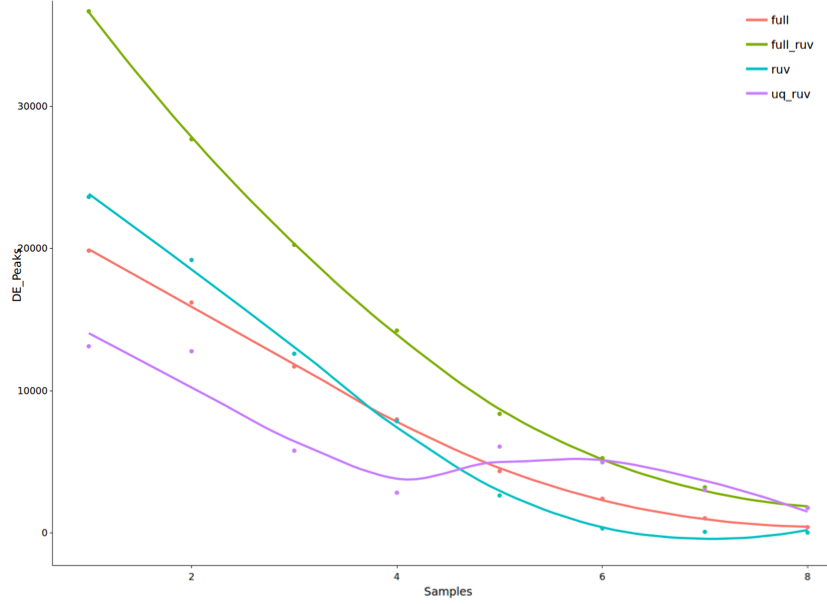
\includegraphics[width=\textwidth, height=\textheight, keepaspectratio]{img/descan2/normalizations.png}
\caption[Normalizations applied to detected regions]{The figure shows the effects of different normalizations on the epigenomic differentially enriched regions.}
\label{fig:normalizationsdescan}
\centering
\end{figure}

To estimate the \glspl{der}, any of the RNA-Seq methods can be applied, such as \textit{DESeq2}, \textit{edgeR}, \textit{NOISeq}, etc \cite{Robinson2009, McCarthy2012, Tarazona2012}.

In this case, we decided to use \textit{edgeR} package, because of its wide range of  available statistical approaches and the possibility to better tune the design of the experiment. 
Indeed, because we used the RUV-Seq normalized counts with \lstinline{k} parameter set to 4, we modeled the experimental design with the \lstinline{model.matrix} function, adding to our model not only the experimental conditions, but also the RUV-Seq estimated weights.
Then we used the resulted design to estimate the dispersion and fit a Quasi-Likelihood test, as defined in edgeR.

The figure \ref{fig:depeaksdescan} shows a volcano plot of \glspl{der} between E0 and E1 conditions.
Red dots highlights the regions with a False Discovery Rate (FDR) lower than 0.05, while blue dots highlight not significant regions.
 
\begin{figure}[h]
\centering
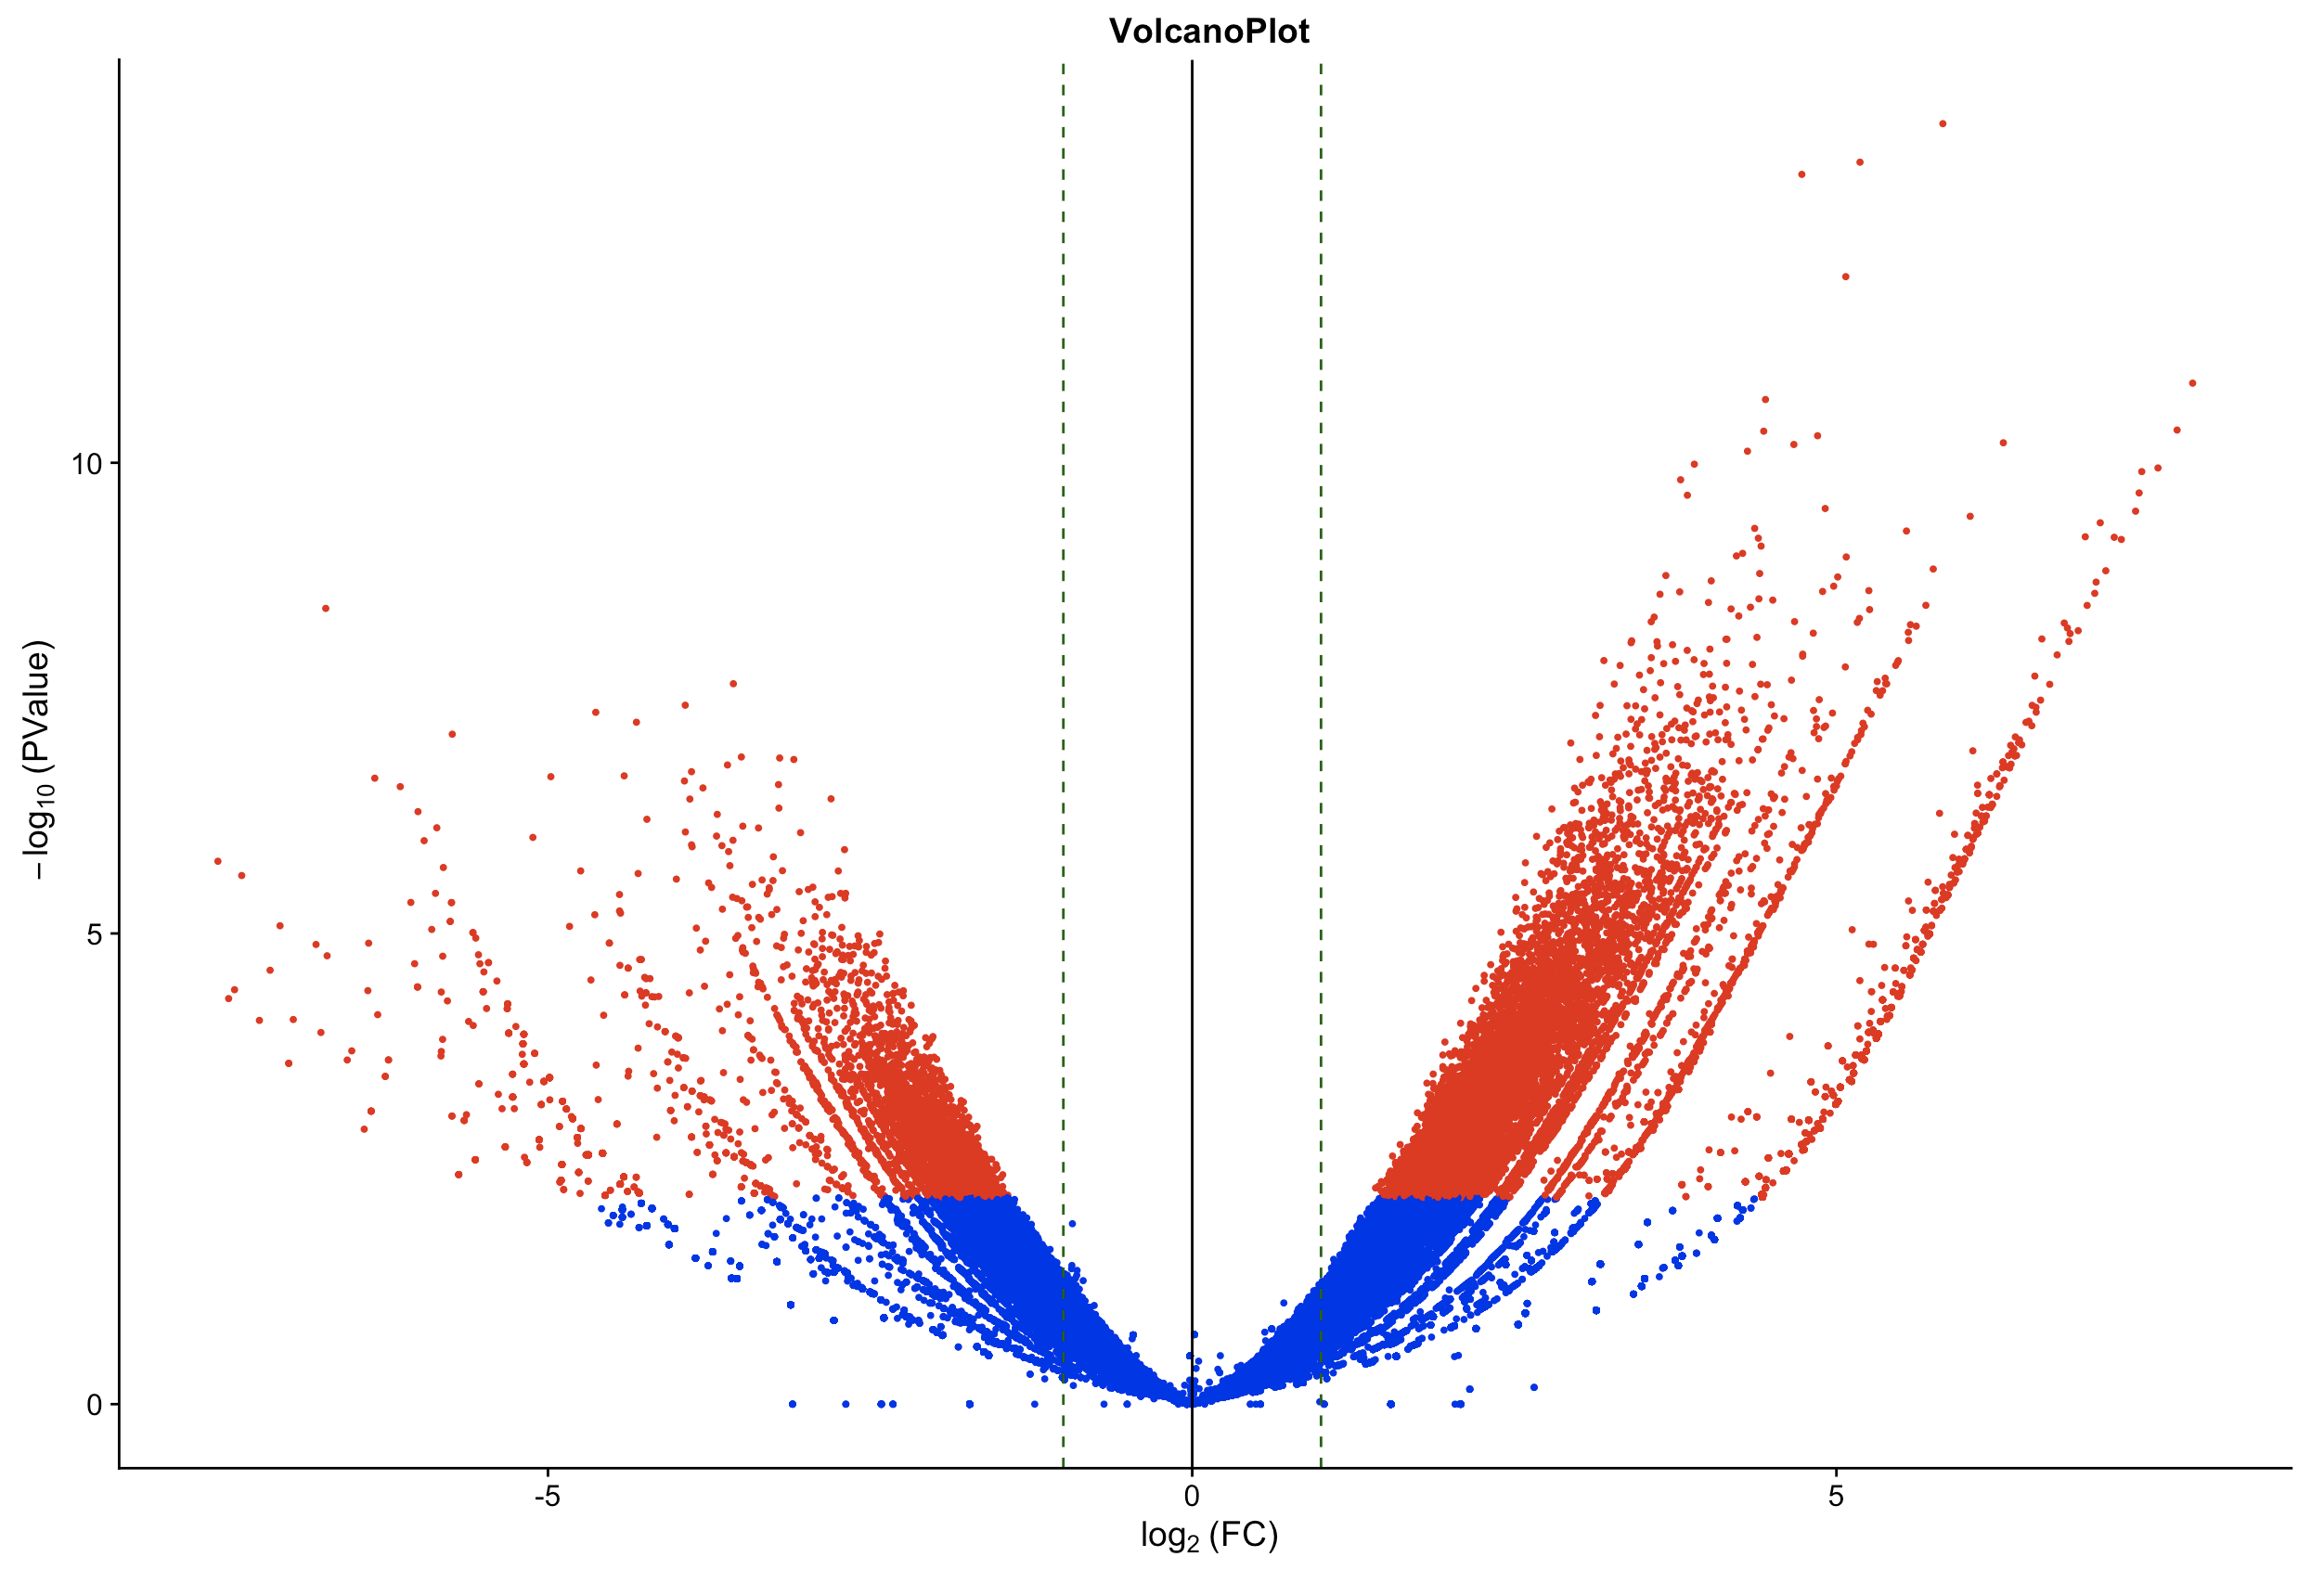
\includegraphics[width=\textwidth, height=\textheight, keepaspectratio]{img/descan2/DE_peaks.png}
\caption[Differential Enrichment Regions Volcano]{A volcano plot of Differential Enriched Regions. Blue dots represent the not significant \glspl{der}, while the red ones represent the significant \glspl{der}.}
\label{fig:depeaksdescan}
\centering
\end{figure}

Next task is to integrate the obtained results with other omic data types, as RNA-Seq. 
Because of the low number of the samples, the easiest way to integrate the data is to annotate the \glspl{der} with differentially expressed genes resulting from the analysis of RNA-Seq.

For the Differential expression of the RNA-Seq data we firstly quantified the signal with \lstinline{featureCounts} methods available in the \textit{Rsubread} \cite{Liao2013} Bioconductor package.
Then we filtered lowly expressed genes with the \textit{proportion} test  as implemented in \textit{NOISeq} package, and applied the \lstinline{noiseq} method for differential expression.%{

\begin{figure}[h]
\centering
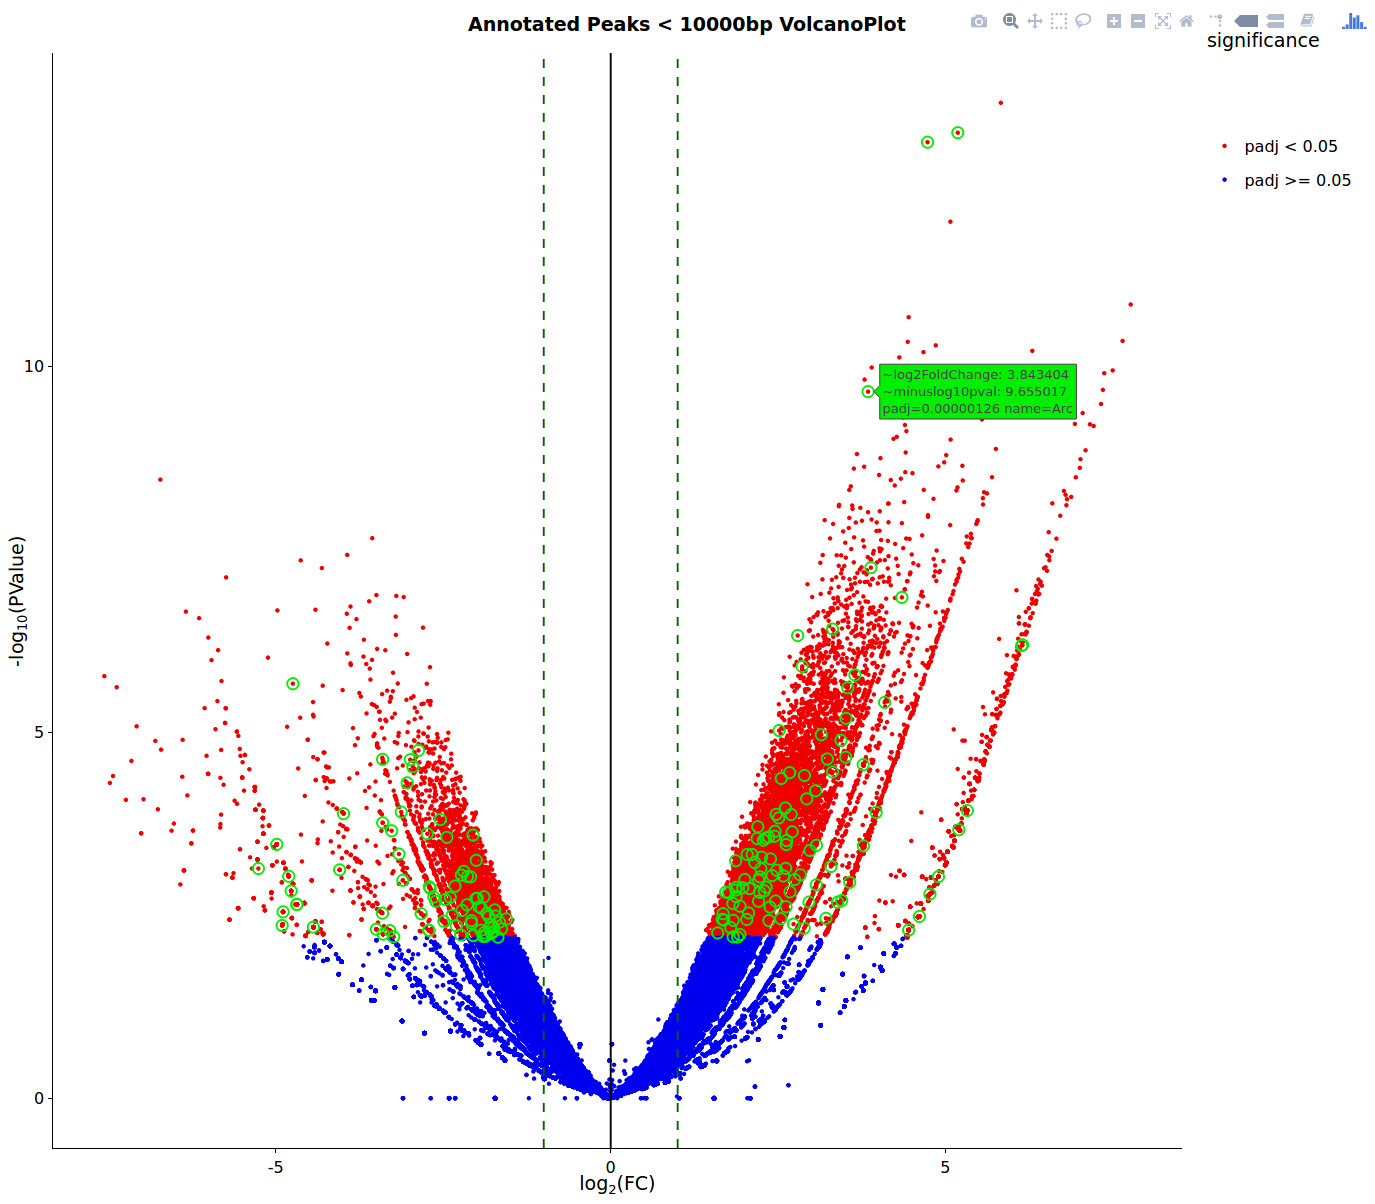
\includegraphics[width=\textwidth, height=\textheight, keepaspectratio]{img/descan2/Annotated_depeaks_degenes.png}
\caption[Annotated Differential Enrichment Regions Volcano]{A volcano plot of \glspl{der}. Blue dots represent the not significant \glspl{der}, while the red ones represent the significant \glspl{der}. Green circles highlights the peaks with a \gls{deg} annotated.}
\label{fig:depeakdegenessdescan}
\centering
\end{figure}

We selected the significant \glspl{deg} with a probability higher than 0.95, and used these genes to annotate the peaks with \lstinline{annotatePeakInBatch} method of ChIPpeakAnno.
Figure 	\ref{fig:depeakdegenessdescan} illustrates with green circles the peaks with an annotated gene with distance lower than 10000bp from the gene TSS.
Realizing the plot with the \textit{plotly} library it's possible to enhance the names of the genes with a tip window.











%%%%%%%%%%%%%%%%%%%%%%%%%%%%%%%%%%%%%%%%%%
\chapter{IntegrHO - Integration of High-Throughtput Omics data}
\section{Introduction}
\section{Methods}
\subsection{Single Omic Approach}
\subsection{Multi Omic Approach}
\subsubsection{Low Level Itegration}
\subsubsection{High Level Itegration}
\section{Implementation Aspects}
\section{Reproducible Computational Research}
\section{Results}

\chapter{Conclusions \& Future Works}


\begin{appendices}
\section{R Language}
\section{R Markdown Language}
%\include{appendixA}
%\include{appendixB}
%\include{appendixC}
\end{appendices}

%This chapter provides all the aspects needed to understand the context of this thesis work, highlighting, moreover, which are the the proposed goals of it.
%explains some basic information useful to understand the context where this thesis work has been developed.

It starts from showing some biological basic aspects and how it is possible to study some cellular behaviours from multiple points of view, using different sequencing techniques and how to integrate them.
Showing, moreover, the importance of keeping trace of the processes involved in the information extraction and why we underlying this aspect. 


%\include{aim_of_the_study}
%\include{MVDA}
%\include{INSIdEnano}
%\include{discussion}
%\include{conclusion}

%\begin{appendices}
%\include{appendixA}
%\include{appendixB}
%\include{appendixC}
%\end{appendices}
%\makeglossaries


\printbibliography[heading=bibnumbered]
\cleardoublepage


\cleardoublepage
% \phantomsection
\addcontentsline{toc}{chapter}{\listfigurename}
\listoffigures

\cleardoublepage
% \phantomsection
\addcontentsline{toc}{chapter}{\listtablename}
\listoftables

%\listoffigures
%\listoftables

\end{document}